\documentclass[12pt,letterpaper]{article}

\usepackage[utf8]{inputenc}
\usepackage{amsmath}
\usepackage{amssymb}
\usepackage{amsfonts}
\usepackage[left=2cm,right=2cm,top=2cm,bottom=2cm]{geometry}
\usepackage{lipsum}
\usepackage{xcolor}
\usepackage{sectsty}
\usepackage{multicol} % para columnas
\usepackage{tcolorbox} % para cajas
\usepackage[all]{xy} % para matrices con flecha (usada para el metodo aspa entre otros)

\usepackage{physics} % para derivadas variables fisicas etc.

% definiendo importador de imagenes
\usepackage{float}
\usepackage{graphicx} % para importar imagenes
\usepackage{cancel} %para cancelar, tachar expresiones (util para la notacion de simplificar)
\usepackage{gensymb} % para grado ej./ 50°

% para graficas y dibujos
\usepackage{tikz,pgfplots}
\usetikzlibrary{matrix} %usar matrices en tikz
% carpeta donde estan la imagenes
\graphicspath{{img/}}
%
%definiendo colores
\definecolor{fuxia}{RGB}{230, 0, 126}
\definecolor{primary}{RGB}{235, 91, 10}
\definecolor{secondary}{RGB}{121, 54, 163}
%
%funte tipografica
\sectionfont{\color{primary}}
\subsectionfont{\color{secondary}}
%
% caja de ejmplo

%
% caja de definicion
\tcbuselibrary{theorems, breakable, skins}
\newtcbtheorem{Theorem}{}%
{
	enhanced, % tcolorbox styles
	%attach boxed title to top center={yshift=-2.5mm},
	colback=white, colframe=fuxia, colbacktitle=white, toprule=0.2mm, leftrule=0.2mm, rightrule=0.2mm, bottomrule=0.2mm , coltitle=fuxia,
	boxed title style={size=small,colframe=white},
	%fonttitle=\bfseries,
	%rounded corners=all,
	toptitle=1ex, top=0.5ex, % a little extra space at top, a little less before content
	titlerule=-1ex, % get rid of separator rule
	title={#1},
	%fontupper=\itshape, % make theorem content italics
	%description delimiters parenthesis, % parentheses around theorem title
	description font=\normalfont,% no bold for theorem title
	separator sign none,% no punctuation after theorem name
	breakable
}{th}
% caja de ejemplo
\newtcbtheorem{Example}{}%
{
	enhanced, % tcolorbox styles
	attach boxed title to top left={yshift=-2.5mm},
	colback=white, colframe=lightgray, colbacktitle=white, toprule=0mm, leftrule=0.8mm, rightrule=0mm, bottomrule=0mm , coltitle=darkgray,
	boxed title style={size=small,colframe=white},
	%fonttitle=\bfseries,
	%rounded corners=all,
	toptitle=1ex, top=0.5ex, % a little extra space at top, a little less before content
	titlerule=-1ex, % get rid of separator rule
	title={#1},
	%fontupper=\itshape, % make theorem content italics
	%description delimiters parenthesis, % parentheses around theorem title
	description font=\normalfont,% no bold for theorem title
	separator sign none,% no punctuation after theorem name
	breakable
}{th}
%
% configurando multicols
\NewEnviron{auxmulticols}[1]{%
	\ifnum#1<2\relax% Fewer than 2 columns
	%\vspace{-\baselineskip}% Possible vertical correction
	\BODY
	\else% More than 1 column
	\begin{multicols}{#1}
		\BODY
	\end{multicols}%
	\fi
}
%
%  definiir seno
\def\sen{\mathop{\mbox{\normalfont sen}}\nolimits}
\def\ctg{\mathop{\mbox{\normalfont ctg}}\nolimits}
\def\tg{\mathop{\mbox{\normalfont tg}}\nolimits}

%para enumeraciones
\renewcommand{\theenumi}{\roman{enumi})}

\author{Franco}

\title{Algo}

\begin{document}
	\begin{multicols}{2}
		\newcounter{exr}
		\setcounter{exr}{0} 
		\section{Matrices}
\subsection{Definición}
La matriz es una forma de ordenamiento rectangular de elementos dispuestos en filas y columnas
\begin{gather*}
	A_{m\cross n}=[a_{ij}]\\
	A=\begin{bmatrix}
		a_{11}&a_{12}&a_{13}&\cdots&a_{1n}\\
		a_{21}&a_{22}&a_{23}&\cdots&a_{2n}\\
		a_{31}&a_{32}&a_{33}&\cdots&a_{3n}\\
		\vdots&\vdots&\vdots&\ddots&\vdots\\
		a_{m1}&a_{m2}&a_{m3}&\cdots&a_{mn}\\
	\end{bmatrix}
\end{gather*}
donde $m$ viene siendo el numero de filas de la matriz y $n$ el numero de columnas.
\subsection{Generación de matrices}
\subsubsection{Matrices cuadradas}
\begin{flalign*}
	&A_{m\cross m} = \begin{bmatrix}
		a_{11} & a_{12} & \cdots & a_{1n} \\
		a_{21} & a_{22} & \cdots & a_{2n} \\
		\vdots & \vdots & \ddots & \vdots \\
		a_{m1} & a_{m2} & \cdots & a_{mn} \\
	\end{bmatrix}
\end{flalign*}
\subsubsection{Matriz delta de Kronecker}
\begin{flalign*}
	&\delta_{n\cross n}=\left[ \ \ \delta_{ij}=\left\{\begin{matrix}
		d & \text{si} & i=j \\
		0 & \text{si} & i\ne j
	\end{matrix}\right. \ \ \right] \\
	&\delta_{n\cross n}=\begin{bmatrix}
		d_{11} & 0 & 0 & \cdots & 0 \\
		0 & d_{22} & 0 & \cdots & 0 \\
		0 & 0 & d_{33} & \cdots & 0 \\
		\vdots & \vdots & \vdots & \ddots & \vdots \\
		0 & 0 & 0 & \cdots & d_{nn}
	\end{bmatrix}
\end{flalign*}
Un caso especial es la matriz identidad:
\begin{flalign*}
	&I_{n\cross n}=\left[ \ \ \delta_{ij}=\left\{\begin{matrix}
		1 & \text{si} & i=j \\
		0 & \text{si} & i\ne j
	\end{matrix}\right. \ \ \right] \\
	&I_{n\cross n}=\begin{bmatrix}
		1 & 0 & 0 & \cdots & 0 \\
		0 & 1 & 0 & \cdots & 0 \\
		0 & 0 & 1 & \cdots & 0 \\
		\vdots & \vdots & \vdots & \ddots & \vdots \\
		0 & 0 & 0 & \cdots & 1
	\end{bmatrix}
\end{flalign*}
\subsubsection{Matriz nulo}
\begin{flalign*}
	&0_{m\cross n}=\left[ \ \ 0_{ij}=0 \ \ \right] \\
	&0_{m\cross n}=\begin{bmatrix}
		0 & 0 & 0 & \cdots & 0 \\
		0 & 0 & 0 & \cdots & 0 \\
		0 & 0 & 0 & \cdots & 0 \\
		\vdots & \vdots & \vdots & \ddots & \vdots \\
		0 & 0 & 0 & \cdots & 0
	\end{bmatrix}
\end{flalign*}
\subsection{Operaciones con Matrices}
\subsubsection{Suma (y resta)}
\begin{flalign*}
	&A + B \\
	&= \begin{bmatrix}
		a_{11} & a_{12} & \cdots & a_{1n} \\
		a_{21} & a_{22} & \cdots & a_{2n} \\
		\vdots & \vdots & \ddots & \vdots \\
		a_{m1} & a_{m2} & \cdot & a_{mn}
	\end{bmatrix} + \begin{bmatrix}
		b_{11} & b_{12} & \cdots & b_{1n} \\
		b_{21} & b_{22} & \cdots & b_{2n} \\
		\vdots & \vdots & \ddots & \vdots \\
		b_{m1} & b_{m2} & \cdot & b_{mn}
	\end{bmatrix} \\
	&= \begin{bmatrix}
		a_{11}+b_{11} & a_{12}+b_{12} & \cdots & a_{1n}+b_{1n} \\
		a_{21}+b_{21} & a_{22}+b_{22} & \cdots & a_{2n}+b_{2n} \\
		\vdots & \vdots & \ddots & \vdots \\
		a_{m1}+b_{m1} & a_{m2}+b_{m2} & \cdot & a_{mn}+b_{mn}
	\end{bmatrix}
\end{flalign*}
\noindent\textbf{\textit{Propiedades de la suma de matrices (C.A.N.I.)}}
\begin{enumerate}
	\item $ A+B=B+A $ (conmutativa)
	\item $ A+(B+C) = (A+B)+C $ (asociativa)
	\item $ A+0=A $ (neutro)
	\item $ A+(-A)=0 $
\end{enumerate}
\subsubsection{Multiplicación por escalar}
\begin{flalign*}
	kA&=k\begin{bmatrix}
		a_{11} & a_{12} & \cdots & a_{1n} \\
		a_{21} & a_{22} & \cdots & a_{2n} \\
		\vdots & \vdots & \ddots & \vdots \\
		a_{m1} & a_{m2} & \cdot & a_{mn}
	\end{bmatrix} \\
	&=\begin{bmatrix}
		ka_{11} & ka_{12} & \cdots & ka_{1n} \\
		ka_{21} & ka_{22} & \cdots & ka_{2n} \\
		\vdots & \vdots & \ddots & \vdots \\
		ka_{m1} & ka_{m2} & \cdot & ka_{mn}
	\end{bmatrix}
\end{flalign*}
\textbf{\textit{Propiedades de multiplicación por escalar}}
\begin{enumerate}
	\item $ k(A+B)=kA+kB $ \\
	$ (k_1+k_2)A=k_1A+k_2A $ (distributiva)
	\item $ (k_1k_2)A=k_1(k_2A) $ (Asociativo)
	\item $ 1\cdot A=A \quad 0\cdot A=0 $ (neutro)
\end{enumerate}
\end{multicols}
\subsubsection{Producto de matrices}
\begin{Theorem*} {Condición para el Producto de matrices}
	Sean las matriz $A_{m\cross n}$ y $B_{p\cross q}$, entonces existe el producto de ambos $A_{m\cross n} \cdot B_{p\cross q}=C_{m\cross q}$ si y solo si $n=p$
	$$ \exists  A_{m\cross n} \cdot B_{p\cross q}=C_{m\cross q} \Leftrightarrow n=p $$
\end{Theorem*}
Esta condición podemos resaltar lo siguiente:
\begin{itemize}
	\item Dos matrices se pueden multiplicar si y solo si, el numero de columnas de la primera matriz es igual al numero de filas de la segunda matriz. $$ A_{m\cross n} \cdot B_{p\cross q}=C_{m\cross q} \Leftrightarrow n=p  $$
	\item Sí el producto $A_{m\cross n} \cdot B_{p\cross q}$ existe, la matriz resultante $C_{m\cross q}$ sera de dimensiones $m\cross q$, es decir tendra el numero de filas de $A$ y el numero de columnas de $B$.
	\item La conmutatividad no existe, es decir se puede multiplicar $A_{2\cross 3} \cdot B_{3\cross 5}=C_{2\cross 5}$ pero no se puede multiplicar $B_{3\cross 5} \cdot A_{2\cross 3}$. Esto nos indica que el producto de matrices no es igual al producto que conocemos de toda la vida, lo cual todo.
\end{itemize}
\textbf{\textit{Proceso practico para multiplicar matrices}} \\
La forma practica para multiplicar matrices es el llamado \textbf{Fila por Columna}:
\begin{flalign*}
	&AB=\begin{bmatrix}
		a_{11} & a_{12} & \cdots & a_{1n} \\
		a_{21} & a_{22} & \cdots & a_{2n} \\
		\vdots & \vdots & \ddots & \vdots \\
		a_{m1} & a_{m2} & \cdots & a_{mn}
	\end{bmatrix}\begin{bmatrix}
		b_{11} & b_{12} & \cdots & b_{1n} \\
		b_{21} & b_{22} & \cdots & b_{2n} \\
		\vdots & \vdots & \ddots & \vdots \\
		b_{m1} & b_{m2} & \cdots & b_{mn}
	\end{bmatrix} \\
	&=\left[\begin{smallmatrix}
		(a_{11}b_{11}+a_{12}b_{21}+\cdots+a_{1n}b_{m1}) & (a_{11}b_{12}+a_{12}b_{22}+\cdots+a_{1n}b_{m2}) & \cdots & (a_{11}b_{1n}+a_{12}b_{2n}+\cdots+a_{1n}b_{mn}) \\
		(a_{21}b_{11}+a_{22}b_{21}+\cdots+a_{2n}b_{m1}) & (a_{21}b_{12}+a_{22}b_{22}+\cdots+a_{2n}b_{m2}) & \cdots & (a_{21}b_{1n}+a_{22}b_{2n}+\cdots+a_{2n}b_{mn}) \\
		\vdots & \vdots & \ddots & \vdots \\
		(a_{m1}b_{11}+a_{m2}b_{21}+a_{mn}b_{m1}) & (a_{m1}b_{12}+a_{m2}b_{22}+\cdots+a_{mn}b_{m2}) & \cdots & (a_{m1}b_{1n}+a_{m2}b_{2n}+\cdots+a_{mn}b_{mn})
	\end{smallmatrix}\right]
\end{flalign*}\\
\addtocounter{exr}{1}
\colorbox{gray!55}{\textcolor{white}{Ej.\arabic{exr}) producto de matrices}}
	Hallar $AB$ si $A=\bigl[\begin{smallmatrix}3 & 5\\ 2 & 1\end{smallmatrix}\bigr]$ y $B=\bigl[\begin{smallmatrix}4 & 7\\ 8 & 9\end{smallmatrix}\bigr]$ \\
\textcolor{gray}{Solución }
	\begin{flalign*}
		AB&=\begin{bmatrix}
			3 & 5 \\
			2 & 1 
		\end{bmatrix}\begin{bmatrix}
			4 & 7 \\
			8 & 9 
		\end{bmatrix}=\begin{bmatrix}
			(3\cdot4 + 5\cdot8) & (3\cdot7+5\cdot9) \\
			(2\cdot4+1\cdot8) & (2\cdot7+1\cdot9)
		\end{bmatrix}=\begin{bmatrix}
			52 & 66 \\
			16 & 23 
		\end{bmatrix}
	\end{flalign*}
\hspace*{\fill}\colorbox{gray!55}{ } \\
\noindent\textbf{\textit{Propiedades del producto de matrices}}
\begin{enumerate}
	\item $AB\ne BA$ (no conmutable)
	\item $(AB)C=A(BC)$ (asociativa)
	\item $A_{m\cross n}I_{n\cross n}=A_{m\cross n}$ (neutro)
	\item La inversa es un caso especial debido a que no existe conmutabilidad:
	\begin{enumerate}
		\item $A_{m\cross n}\cdot A_{n\cross m}^-1=I_{m\cross m}$ (por derecha o postmultiplica)
		\item $A_{n\cross m}^-1\cdot A_{m\cross n}=I_{n\cross n}$ (por izquierda o premultiplica) \\
		Son diferentes por eso se llama pseudoinversas, unicamente cuando la matriz es cuadrada la inversa es unica:
		\item $A_{n\cross n}\cdot A_{n\cross n}^-1=A_{n\cross n}^-1\cdot A_{n\cross n}=I_{n\cross n}$
	\end{enumerate}
	\item $A(B+C)=AB+AC$ (ley distributiva por la izquierda o premultiplica)
	\item $(B+C)A=BA+CA$ (ley distributiva por la derecha o postmultiplica)
\end{enumerate}
\begin{multicols}{2}
\subsection{Otras operaciones de matrices}
\subsubsection{Matriz transpuesta}
\begin{Theorem*} {Matriz transpuesta}
	La transpuesta de una matriz $A$, denotada por $A^T$, es la matriz obtenida escribiendo las filas de $A$ por orden como columnas:
	$$ A_{m\cross n} = [a_{ij}] \rightarrow A^T_{n\cross m} = [a_{ji}] $$
\end{Theorem*}
Es decir las filas de $A$ pasan a ser columnas de $A^T$ y las columnas de $A$ pasa ser filas de $A^T$. \\\\
\addtocounter{exr}{1} 
\colorbox{gray!55}{\textcolor{white}{Ej.\arabic{exr}) matriz transpuesta}}
	Hallar la transpuesta de $A=\left[\begin{smallmatrix}
		3 & -4 \\
		5 & 6 \\
		2 & 8 
	\end{smallmatrix}\right]$\\
\textcolor{gray}{Solución }
	\begin{flalign*}
		A_{3\cross2}=\begin{bmatrix}
			3 & -4 \\
			5 & 6 \\
			2 & 8
		\end{bmatrix} \\
		\therefore A^T_{2\cross3}=\begin{bmatrix}
			3 & 5 & 2 \\
			-4 & 6 & 8
		\end{bmatrix}
	\end{flalign*}
\hspace*{\fill}\colorbox{gray!55}{ } \\
\noindent\textbf{\textit{Propiedades de una matriz transpuesta}}
\begin{enumerate}
	\item $ (A+B)^T=A^T+B^T $
	\item $ (A^T)^T=A $
	\item $ (kA)^T=kA^T $ (k: escalar)
	\item $ (AB)^T=A^TB^T $
\end{enumerate}
\subsubsection{Traza de una matriz}
La traza es una operacion donde interviene la diagonal principal
\begin{Theorem*} {Traza de una matriz}
	Sea $A_{n\cross n=[a_{ij}]}$ entonces su traza denotada por $tr(A)$ se define de la siguiente manera:
	$$ tr(A)=\sum_{i=1}^{n}aii $$
\end{Theorem*}
Es decir, que la traza viene siendo la suma de los elementos de la diagonal principal de una matriz cuadrada. \\\\
\addtocounter{exr}{1} 
\colorbox{gray!55}{\textcolor{white}{Ej.\arabic{exr}) traza de una matriz}}
	Hallar la traza de $A$
	$$A=\begin{bmatrix}
		2 & 1 & 3 \\
		4 & 2 & 5 \\
		0 & 0 & -1
	\end{bmatrix}$$
\textcolor{gray}{Solución }
	\begin{flalign*}
		&A=\begin{bmatrix}
			2 & 1 & 3 \\
			4 & 2 & 5 \\
			0 & 0 & -1
		\end{bmatrix} \\
		&tr(A)=2+2+(-1) \\
		&\therefore tr(A)=3
	\end{flalign*}
\hspace*{\fill}\colorbox{gray!55}{ }
\subsection{Operaciones y tipos especiales de matrices cuadradas}
\subsubsection{Matriz diagonal}
La matriz diagonal se define de la siguiente manera:
\begin{Theorem*} {Matriz diagonal}
	Es aquella matriz donde sus entradas no diales son nulaes, por lo tanto cumple que:
	$$
		A_{n\cross n}=\left[ \ \ a_{ij}=\left\{\begin{matrix}
			a_{ii} & si & i=j \\
			0 & si & i\ne j
		\end{matrix}\right. \ \ \right]
	$$
\end{Theorem*}
Es decir son aquellas matrices donde solo tienen valoes en la diagonal principal
$$
	A_{n\cross n}=\begin{bmatrix}
		a_{11} & 0 & 0 & \cdots & 0 \\
		0 & a_{22} & 0 & \cdots & 0 \\
		0 & 0 & a_{33} & \cdots & 0 \\
		\vdots & \vdots & \vdots & \ddots & \vdots \\
		0 & 0 & 0 & \cdots & a_{nn}
	\end{bmatrix}
$$
\subsubsection{Matriz Triangular}
\begin{Theorem*} {Matriz Triangular}
	Son aquellas matrices donde sus entradas por encima o por debajo de su diagonal principal son nulas y debido a esta condicion pueden ser superio o inferior respectivamente.
	\begin{itemize}
		\item matriz triangula superior
		$$A_{n\cross n}=\left[ \ \ a_{ij}=\left\{\begin{matrix}
			a_{ij} & si & i\le j \\
			0 & si & i>j
		\end{matrix}\right. \ \ \right]$$
		\item matriz triangula superior
		$$A_{n\cross n}=\left[ \ \ a_{ij}=\left\{\begin{matrix}
			a_{ij} & si & i\ge j \\
			0 & si & i<j
		\end{matrix}\right. \ \ \right]$$
	\end{itemize}
\end{Theorem*}
Tambien a este tipo de matrices se las denominan matrices escalonadas por forma escalones
$$
	A_{4\cross 4}=\begin{bmatrix}
		a_{11} & a_{12} & a_{13} & a_{14} \\
		0 & a_{22} & a_{23} &  a_{24} \\
		0 & 0 & a_{33} &  a_{34} \\
		0 & 0 & 0  & a_{44}
	\end{bmatrix}
$$
$$
B_{4\cross 4}=\begin{bmatrix}
	b_{11} & 0 & 0 & 0 \\
	b_{21} & b_{22} & 0 &  0 \\
	b_{31} & b_{32} & b_{33} &  0 \\
	b_{41} & b_{42} & b_{43}  & b_{44}
\end{bmatrix}
$$
\subsubsection{Potencia de una matriz}
\begin{Theorem*} {Potencia de una matriz}
	Si la matriz $A$ es cuadrada entonces se puede multiplicar por si misma n veces:
	$$ A^n=A\cdot A\cdot A\cdot \cdots \cdot A $$
\end{Theorem*}
Por lo tanto, para poder sacar la potencia de una matriz, debes saber cómo resolver una multiplicación de matrices. De lo contrario, no puedes calcular una potencia matricial. \\\\
\addtocounter{exr}{1} 
\colorbox{gray!55}{\textcolor{white}{Ej.\arabic{exr}) potencia de una matriz}}
	Hallar $A^2$, $A^3$ y $A^4$
	$$ A=\begin{bmatrix}
		1 & -1 \\
		1 & 0
	\end{bmatrix} $$
\textcolor{gray}{Solución }
	\begin{align*}
		&A^2=AA=\begin{bmatrix}
			1 & -1 \\
			1 & 0
		\end{bmatrix}\begin{bmatrix}
			1 & -1 \\
			1 & 0
		\end{bmatrix}=\begin{bmatrix}
			0 & -1 \\
			1 & -1
		\end{bmatrix} \\
		&A^3=A^2A=\begin{bmatrix}
			0 & -1 \\
			1 & -1
		\end{bmatrix}\begin{bmatrix}
			1 & -1 \\
			1 & 0
		\end{bmatrix}=\begin{bmatrix}
			-1 & 0 \\
			0 & -1
		\end{bmatrix} \\
		&A^4=A^3A=\begin{bmatrix}
			-1 & 0 \\
			0 & -1
		\end{bmatrix}\begin{bmatrix}
			1 & -1 \\
			1 & 0
		\end{bmatrix}=\begin{bmatrix}
			-1 & 1 \\
			-1 & 0
		\end{bmatrix}
	\end{align*}
\hspace*{\fill}\colorbox{gray!55}{ } \\
Con esta operacion podemos ver algunas matrices especiales:
\begin{enumerate}
	\item \textbf{\textit{Matriz idempotente}}
	Es aquella matriz cuadrada que multiplicada por ella misma da como resultado la misma matriz:
	$$ A^2 = A $$
	\item  \textbf{\textit{Matriz involutiva}}
	Es aquella matriz cuadrada que multiplicada por ella misma da como resultado la matriz identidad:
	$$ A^2 = I $$
	Debido que al multiplicarse da la identidad, también se puede definirse como una matriz invertible:
	$$ A^{-1} = A $$
	Así que, evidentemente, una matriz involutiva es un ejemplo de matriz regular o no degenerada.
	\item \textbf{\textit{Matriz nilpotente}}
	Es una matriz cuadrada que elevada a algún número entero da como resultado la matriz nula.
	$$ A^n=0 $$
	\item \textbf{\textit{Matriz periódica}}
	Es aquella matriz cuya potencia $(k+1)$ da como resultado la misma matriz:
	$$ A^{k+1}=A $$ $$ k\in \mathbb{R}, k: \text{periodo de la matriz} $$
	note que si la matriz es peridica de para $k=1$ (orden 1) entonces es una matriz idempotente.
\end{enumerate}
\addtocounter{exr}{1} 
\colorbox{gray!55}{\textcolor{white}{Ej.\arabic{exr}) matriz periódica}}
	Demostrar que la matriz $A$ es periódica de grado $6$
	$$ A=\begin{bmatrix}
		1 & -1 \\
		1 & 0
	\end{bmatrix} $$
\textcolor{gray}{Solución }
	\begin{align*}
		&A^2=AA=\begin{bmatrix}
			1 & -1 \\
			1 & 0
		\end{bmatrix}\begin{bmatrix}
			1 & -1 \\
			1 & 0
		\end{bmatrix}=\begin{bmatrix}
			0 & -1 \\
			1 & -1
		\end{bmatrix} \\
		&A^3=A^2A=\begin{bmatrix}
			0 & -1 \\
			1 & -1
		\end{bmatrix}\begin{bmatrix}
			1 & -1 \\
			1 & 0
		\end{bmatrix}=\begin{bmatrix}
			-1 & 0 \\
			0 & -1
		\end{bmatrix} \\
		&A^4=A^3A=\begin{bmatrix}
			-1 & 0 \\
			0 & -1
		\end{bmatrix}\begin{bmatrix}
			1 & -1 \\
			1 & 0
		\end{bmatrix}=\begin{bmatrix}
			-1 & 1 \\
			-1 & 0
		\end{bmatrix} \\
		&A^5=A^4A=\begin{bmatrix}
			-1 & 1 \\
			-1 & 0
		\end{bmatrix}\begin{bmatrix}
			1 & -1 \\
			1 & 0
		\end{bmatrix}=\begin{bmatrix}
			0 & 1 \\
			-1 & 1
		\end{bmatrix} \\
		&A^6=A^5A=\begin{bmatrix}
			0 & 1 \\
			-1 & 1
		\end{bmatrix}\begin{bmatrix}
			1 & -1 \\
			1 & 0
		\end{bmatrix}=\begin{bmatrix}
			1 & 0 \\
			0 & 1
		\end{bmatrix} = I \\
		&A^7=A^6A=IA=A
	\end{align*}
\hspace*{\fill}\colorbox{gray!55}{ } \\
\begin{Example*} {Matriz periodica - ejemplo 2}
	Sea $A$ una matriz cuadrada, periódica de grado 3 y se sabe que $A^3=I$; hallar $A^{100}$
	Sol.
	\begin{flalign*}
		&A^3=I; \text{periódica de grado 3: }A^4=A;\\
		&A^{100}=? \\
		&A^3=I\\
		&A^4=IA=A \\
		&A^5=A^4A=AA=A^2 \\
		&A^6=A^5A=A^2A=A^3=I \\
		&A^7=A^6A=IA=A \\
		&A^8=A^7A=AA=A^2 \\
		&A^9=A^8A=A^2A=A^3=I\\
		&\quad \vdots \\
		&\text{note que elevado a un múltiplo de 3 es I} \\
		&\quad \vdots \\
		&A^{99}=I\\
		&A^{100}=A^{99}A=IA=A\\
		&\therefore \ A^{100}=A
	\end{flalign*}
\end{Example*}
\subsubsection{Matrices simétricas}
\begin{Theorem*} {Matriz simétrica}
	Se llama matriz simétrica si esta es igual a su traspuesta
	$$ A=A^T $$
\end{Theorem*}
La matriz simétrica también se la nombra como matriz simétricamente. Así también, se llama anti simétrica si esta es igual a su transpuesta pero con signo cambiado.
$$ A=-A^T $$
\addtocounter{exr}{1} 
\colorbox{gray!55}{\textcolor{white}{Ej.\arabic{exr}) matriz simétrica}}
	Demostrar que $A$ es una matriz simétrica
	$$ A=\begin{bmatrix}
		3 & 2 & 1 \\
		2 & 5 & -4 \\
		1 & -4 & -6
	\end{bmatrix} $$
\textcolor{gray}{Solución }
	\begin{align*}
		&A=\begin{bmatrix}
			3 & 2 & 1 \\
			2 & 5 & -4 \\
			1 & -4 & -6
		\end{bmatrix}=A^T=\begin{bmatrix}
		3 & 2 & 1 \\
		2 & 5 & -4 \\
		1 & -4 & -6
		\end{bmatrix}
	\end{align*}
\hspace*{\fill}\colorbox{gray!55}{ } \\
\addtocounter{exr}{1} 
\colorbox{gray!55}{\textcolor{white}{Ej.\arabic{exr}) matriz antisimétrica}}
	Demostrar que $A$ es una matriz anti simétrica
	$$ A=\begin{bmatrix}
		0 & 5 & -4 \\
		-5 & 0 & 6 \\
		4 & -6 & 0
	\end{bmatrix} $$
\textcolor{gray}{Solución }
	\begin{align*}
		&A=\begin{bmatrix}
			0 & 5 & -4 \\
			-5 & 0 & 6 \\
			4 & -6 & 0
		\end{bmatrix}=A^T=\begin{bmatrix}
			0 & -5 & 4 \\
			5 & 0 & -6 \\
			-4 & 6 & 0
		\end{bmatrix}
	\end{align*}
\hspace*{\fill}\colorbox{gray!55}{ } \\
Propiedades:
\begin{enumerate}
	\item en toda matriz antisimetrica se cumple:
	$$ A_{ii} = 0 $$
\end{enumerate}
\subsubsection{Matrices ortogonales}
\begin{Theorem*} {Matrices ortogonales}
	Sea una A una matriz cuadrada entonces decimos que es ortogonal si:
	$$
	\left.\begin{array} {cc}
		AA^T=I \\
		A^TA=I
	\end{array}\right\}\Longrightarrow A^T=A^{-1}
	$$
\end{Theorem*}
Así también, una matriz ortogonal es una matriz cuadrada con números reales que multiplicada por su traspuesta (o transpuesta) es igual a la matriz Identidad. Es decir, se cumple la siguiente condición:
$$ AA^T=A^TA=I $$ \\
\addtocounter{exr}{1} 
\colorbox{gray!55}{\textcolor{white}{Ej.\arabic{exr}) matrices ortogonales}}
	Demostrar que $A$ es una matriz ortogonal
	$$ A=\begin{bmatrix}
		1/9 & 8/9 & -4/9 \\
		4/9 & -4/9 & -7/9 \\
		8/9 & 1/9 & 4/9
	\end{bmatrix} $$
\textcolor{gray}{Solución }
	\begin{align*}
		&AA^T=I \\
		&\begin{bmatrix}
			1/9 & 8/9 & -4/9 \\
			4/9 & -4/9 & -7/9 \\
			8/9 & 1/9 & 4/9
		\end{bmatrix}\begin{bmatrix}
			1/9 & 4/9 & 8/9 \\
			8/9 & -4/9 & 1/9 \\
			-4/9 & -7/9 & 4/9
		\end{bmatrix} \\
		&=1/81\left[\begin{smallmatrix}
			(1+64+16) & (4-32+28) & (8+8-16) \\
			(4-32+28) & (16+16+49) & (32-4-28) \\
			(8+8-16) & (32-4-28) & (64+1+16)
		\end{smallmatrix}\right] \\
		&1/81\begin{bmatrix}
			81 & 0 & 0 \\
			0 & 81 & 0 \\
			0 & 0 & 81
		\end{bmatrix} = \begin{bmatrix}
			1 & 0 & 0 \\
			0 & 1 & 0 \\
			0 & 0 & 1
		\end{bmatrix} = I \\
		&\therefore \ A \text{ es ortogonal}
	\end{align*}
\hspace*{\fill}\colorbox{gray!55}{ } \\
\subsection{Operaciones elementales (O.E.)}
Son cambios que se pueden realizar en las filas y/o columnas de una matriz con el objetivo de encontrar una matriz equivalente
\begin{enumerate}
	\item Intercambiar dos filas o columnas
	\begin{gather*}
		f_i\leftrightarrow f_j \\
		c_i\leftrightarrow c_j
	\end{gather*}
	\item Multiplicar por un escalar una fila o columna no nulo
	\begin{gather*}
		kf_i\rightarrow f_i \\
		kc_i\rightarrow c_i
	\end{gather*}
	\item suma una fila o columna k veces a otra
	\begin{gather*}
		kf_i+f_j\rightarrow f_j \\
		kc_i+c_j\rightarrow c_j
	\end{gather*} 
\end{enumerate}
\addtocounter{exr}{1} 
\colorbox{gray!55}{\textcolor{white}{Ej.\arabic{exr}) O.E. reduc
		ción a escalonada}}
	Reducir $A$, a una forma escalonada
	$$ A=\begin{bmatrix}
		1 & 2 & -3 & 0 \\
		2 & 4 & -2 & 2 \\
		3 & 6 & -4 & 3
	\end{bmatrix} $$
\textcolor{gray}{Solución }
	\begin{align*}
		&\begin{array} {c}
			=\begin{bmatrix}
				1 & 2 & -3 & 0 \\
				2 & 4 & -2 & 2 \\
				3 & 6 & -4 & 3
			\end{bmatrix} \\
			-2f_1+f_2\rightarrow f_2
		\end{array}
		\begin{array} {c}
			\sim\begin{bmatrix}
				1 & 2 & -3 & 0 \\
				0 & 0 & 4 & 2 \\
				3 & 6 & -4 & 3
			\end{bmatrix} \\
			-3f_1+f_3\rightarrow f_3
		\end{array} \\
		&\begin{array} {c}
			\sim\begin{bmatrix}
				1 & 2 & -3 & 0 \\
				0 & 0 & 4 & 2 \\
				0 & 0 & 5 & 3
			\end{bmatrix} \\
			4f_3\rightarrow f_3
		\end{array}
		\begin{array} {c}
			\sim\begin{bmatrix}
				1 & 2 & -3 & 0 \\
				0 & 0 & 4 & 2 \\
				0 & 0 & 20 & 12
			\end{bmatrix} \\
			-5f_2+f_3\rightarrow f_3
		\end{array} \\
		&\begin{array} {c}
			A\sim\begin{bmatrix}
				1 & 2 & -3 & 0 \\
				0 & 0 & 4 & 2 \\
				0 & 0 & 0 & 2
			\end{bmatrix}
		\end{array}
	\end{align*}
\hspace*{\fill}\colorbox{gray!55}{ } \\
\subsubsection*{Consecuencia de operaciones elementales}
Cuando se trata un matriz con operaciones elementales, se obtiene una matriz distinta a la original y esta puede ser matriz elemental o equivalente: \\
\textbf{\textit{Matriz elemental}}, es aquella que se obtiene al aplicar una sola operación elemental sobre una matriz identidad.
\begin{align*}
	&\begin{array} {c}
		\begin{bmatrix}
			1&0\\
			0&1
		\end{bmatrix}\\
		2f_1\rightarrow f_1
	\end{array}\sim\begin{bmatrix}
		2&0\\
		0&1
	\end{bmatrix}=E=\text{matriz elemental}
\end{align*}
\textbf{\textit{Matriz equivalente}}, es aquella que se obtiene al aplicar una o mas operaciones elementales a la original.
\begin{align*}
	&A=\begin{array} {c}
		\begin{bmatrix}
			1&2\\
			4&0
		\end{bmatrix}\\
		f_1\leftrightarrow f_2
	\end{array}\sim\begin{bmatrix}
		4&0\\
		1&2
	\end{bmatrix}=B\\
	&\Rightarrow A\sim B (\text{A  y B son equivalentes})
\end{align*}
\textbf{\textit{matrices mas comunes}} \\
Cuando se realiza operaciones elementales a una matriz, casi siempre se el objetivo sera llegar a las siguientes matrices:
\begin{itemize}
	\item Matriz triangular superior o forma escalonada
	$$
	\begin{bmatrix}
		2&7&0\\
		0&5&6\\
		0&0&1
	\end{bmatrix} \text{ ó } \begin{bmatrix}
		1&2&5&3\\
		0&5&9&1\\
		0&0&3&1
	\end{bmatrix}
	$$
	\item  Matriz triangular inferior
	$$
	\begin{bmatrix}
		1&0&0\\
		5&-1&0\\
		3&2&3
	\end{bmatrix} \text{ ó } \begin{bmatrix}
		2&0&0\\
		5&-4&0\\
		8&3&1\\
		9&2&8
	\end{bmatrix}
	$$
	\item Forma escalonada reducida (Matriz identidad)\\
	una matriz a la cual se quiere llegar siempre es la matriz identidad, debido que es la forma mas comun de hallar la inversa, es decir si se llega a la identidad entonces existe la inversa de la matriz que se transformó
	$$
	\begin{bmatrix}
		1&0&0\\
		0&1&0\\
		0&0&1
	\end{bmatrix}
	$$
	sin embargo si esto no es posible y se llega a algo como esto:
	$$
	\begin{bmatrix}
		1&0&0\\
		0&1&0\\
		0&0&0
	\end{bmatrix}
	$$
	entonces concluimos que la matriz no tiene inversa
\end{itemize}
\subsubsection{Estrategias para reducir y transformación matrices}
Las operaciones elementales son útiles para transformar a una matriz equivalente deseada. \\
\textbf{\textit{Transformar a una matriz identidad equivalente}}
\begin{enumerate}
	\item \textit{Se busca el pivote}, en la primera columna, esta debe ser 1 sino se debe realizar una operación elemental para obtenerlo.
	\item \textit{Crear ceros}, a partir del pivote en la columna en la que se trabaja.
	\item \textit{Cambiar a la siguiente columna}, y buscar el pivote que ahora siempre debe ser el que tiene mas ceros a la izquierda, el pivote debe ser 1 sino realizar una operación elemental para obtenerlo. Realizar el paso 2.
	\item \textit{Repetir}, el paso 3 hasta que se llegue a la ultima columna (nota: si se trabaja en las primera columnas de la izquierda abra varios pivotes, escoger cualquier o el mas conveniente; a medida que se llegue a la ultima columna el numero de pivotes disminuye has ser uno solo).
	\item \textit{Ordenar}, para que tenga la forma de una matriz identidad
\end{enumerate}
\addtocounter{exr}{1} 
\colorbox{gray!55}{\textcolor{white}{Ej.\arabic{exr}) O.E. reducción a identidad}}
	Reducir a identidad:
	$$
	A=\begin{bmatrix}
		3 & 2 & 0 \\
		4 & 1 & 2 \\
		0 & 4 & 1
	\end{bmatrix}
	$$
\textcolor{gray}{Solución }
	\begin{flalign*}
		&=\begin{bmatrix}
			3 & 2 & 0 \\
			4 & 1 & 2 \\
			0 & 4 & 1
		\end{bmatrix} \begin{matrix}
			(\text{creando pivote en} \\
			\text{columna 1}) \\
			-f_1+f_2\rightarrow f_2
		\end{matrix} \\
		&\sim\begin{bmatrix}
			3 & 2 & 0 \\
			\framebox[0.5cm]{1} & -1 & 2 \\
			0 & 4 & 1
		\end{bmatrix}\begin{matrix}
			(\text{creando ceros en}\\
			\text{columna 1})\\
			-3f_2+f_1\rightarrow f_1
		\end{matrix} \\
		&\sim\begin{bmatrix}
			0 & 5 & -6 \\
			1 & -1 & 2 \\
			0 & 4 & 1
		\end{bmatrix}\begin{matrix}
			(\text{Creando pivote en}\\
			\text{columna 2})\\
			-f_3+f_1\rightarrow f_1
		\end{matrix} \\
		&\sim\begin{bmatrix}
			0 & \framebox[0.5cm]{1} & -7 \\
			1 & -1 & 2 \\
			0 & 4 & 1
		\end{bmatrix}\begin{matrix}
			(\text{Creando ceros en}\\
			\text{columna 2})\\
			f_1+f_2\rightarrow f_2\\
			-4f_1+f_3->f_3
		\end{matrix} \\
		&\sim\begin{bmatrix}
			0 & 1 & -7 \\
			1 & 0 & -5 \\
			0 & 0 & -10
		\end{bmatrix}\begin{matrix}
			(\text{Creando pivote en}\\
			\text{columna 3})\\
			-\frac{1}{10}f_3\rightarrow f_3
		\end{matrix} \\
		&\sim\begin{bmatrix}
			0 & 1 & -7 \\
			1 & 0 & -5 \\
			0 & 0 & \framebox[0.5cm]{1}
		\end{bmatrix}\begin{matrix}
			(\text{Creando ceros en}\\
			\text{columna 3})\\
			7f_3+f_1\rightarrow f_1\\
			5f_3+f_2\rightarrow f_2
		\end{matrix} \\
		&\sim\begin{bmatrix}
			0 & 1 & 0 \\
			1 & 0 & 0 \\
			0 & 0 & 1
		\end{bmatrix}\begin{matrix}
			(\text{ordenando})\\
			f_1\leftrightarrow f_2
		\end{matrix} \\
		&\therefore  A\sim\begin{bmatrix}
			1 & 0 & 0 \\
			0 & 1 & 0 \\
			0 & 0 & 1
		\end{bmatrix}
	\end{flalign*}
\hspace*{\fill}\colorbox{gray!55}{ } \\
\textbf{\textit{Reducccion a un matriz escalonada equivalente}} \\
Los pasos son parecidos a la anterior reducción, solo cambia la forma de encontrar el pivote y ya no cambia todas las entradas a ceros 
\begin{enumerate}
	\item \textit{Se busca el pivote}, esta siempre debe estar en la primera columna y en la primera fila, y esta puede ser cualquier numero excepto el cero.
	\item \textit{Crear ceros}, a partir del pivote en la columna en la que se trabaja, estos ceros deben estar estar por debajo del pivote.
	\item \textit{Cambiar a la siguiente columna}, y buscar el pivote que debe estar en la misma fila o una fila por debajo del anterior pivote.
	\item \textit{Repetir}, el paso 3 hasta que se llegue a la ultima columna
\end{enumerate}
\addtocounter{exr}{1} 
\colorbox{gray!55}{\textcolor{white}{Ej.\arabic{exr}) O.E. reducir a escalonada}}
	Reducir $A$ a escalonada
	$$ A=\begin{bmatrix}
		7&4&1&0 \\
		3&2&0&1 \\
		3&3&2&2
	\end{bmatrix} $$
\textcolor{gray}{Solución }
	\begin{flalign*}
		&=\begin{bmatrix}
			7&4&1&0 \\
			3&2&0&1 \\
			4&3&2&2
		\end{bmatrix} \begin{matrix}
			(\text{buscar pivote en} \\
			\text{columna 1})
		\end{matrix} \\
		&\sim\begin{bmatrix}
			\framebox[0.5cm]{7}&4&1&0 \\
			3&2&0&1 \\
			4&3&2&2
		\end{bmatrix} \begin{matrix}
			(\text{Crear ceros por debajo} \\
			\text{del pivote en columna 1}) \\
			-\frac{3}{7}f_1+f_2\rightarrow f_2\\
			-\frac{4}{7}f_1+f_3\rightarrow f_3
		\end{matrix} \\
		&\sim\begin{bmatrix}
			7&4&1&0 \\
			0&2/7&-3/7&1 \\
			0&5/7&10/7&2
		\end{bmatrix} \begin{matrix}
			(\text{Buscar el pivote} \\
			\text{en columna 2})
		\end{matrix} \\
		&\sim\begin{bmatrix}
			7&4&1&0 \\
			0&\framebox[0.8cm]{2/7}&-3/7&1 \\
			0&5/7&10/7&2
		\end{bmatrix} \begin{matrix}
			(\text{Crear ceros por} \\
			(\text{encima del pivote} \\
			\text{en columna 2}) \\
			-\frac{5}{2}f_2+f_3\rightarrow f_3
		\end{matrix} \\
		&\sim\begin{bmatrix}
			7&4&1&0 \\
			0&2/7&-3/7&1 \\
			0&0&5/2&-1/2
		\end{bmatrix} \begin{matrix}
			(\text{Buscar el pivote} \\
			\text{en columna 3})
		\end{matrix} \\
		&\therefore A\sim\begin{bmatrix}
			7&4&1&0 \\
			0&2/7&-3/7&1 \\
			0&0&5/2&-1/2
		\end{bmatrix}
	\end{flalign*}
\hspace*{\fill}\colorbox{gray!55}{ } \\
\subsubsection{Relación de semejanza de matrices}
Se sabe que si se realiza operaciones elementales a $A$ se obtiene $B$ y se cumple que $A\sim B$; note que $A$ es diferente a $B$ ($A\ne B$), entonces la pregunta ¿existe una relacion matricial entre ambos?, y la respuesta es si:
\begin{Theorem*} {}
	Sea $B$ una matriz obtenido mediante operaciones elementales a $A$:
	$$A_{m\cross n}\sim B_{m\cross n}$$
	por lo tanto existe una relación de equivalencia $P$ y $Q$, entre $A$ y $B$ de la forma:
	$$ P_{m\cross m}\cdot A_{m\cross n}\cdot Q_{n\cross n}=B_{m\cross n} $$
\end{Theorem*}
donde $P$ es el producto de matrices elementales en fila y $Q$ es el producto de matrices elementales en columna, es decir: \\
\begin{gather*}
	P=E_n\cdot E_{n-1}\cdot E_{n-2}\cdot...\cdot E_2\cdot E_1\\
	Q=D_1\cdot D_2\cdot D_3\cdot...\cdot D_{n-1}\cdot D_n
\end{gather*}
Ademas:
$$
	E_0=\left[\begin{smallmatrix}
		1&0&0&\cdots&0\\
		0&1&0&\cdots&0\\
		0&0&1&\cdots&0\\
		\vdots&\vdots&\vdots&\ddots&\vdots\\
		0&0&0&\cdots&1
	\end{smallmatrix}\right] \quad\quad D_0=\left[\begin{smallmatrix}
		1&0&0&\cdots&0\\
		0&1&0&\cdots&0\\
		0&0&1&\cdots&0\\
		\vdots&\vdots&\vdots&\ddots&\vdots\\
		0&0&0&\cdots&1
	\end{smallmatrix}\right]
$$\\
\addtocounter{exr}{1} 
\colorbox{gray!55}{\textcolor{white}{Ej.\arabic{exr}) relación de semejanza de matrices}}
	Hallar la relación Q,Q de las matrices A y B, luego de realizar 3 operaciones elementales en fila y 2 en columna
	$$ A=\begin{bmatrix}
		3&4&1&2\\
		2&0&5&0\\
		1&3&2&1
	\end{bmatrix} $$ \\
\textcolor{gray}{Solución }\\
Se realiza 3 y 2, operaciones elementales en fila y columna cualesquiera, respectivamente:
	\begin{align*}
		&\begin{array} {c}
			A=\begin{bmatrix}
				3&4&1&2\\
				2&0&5&0\\
				1&3&2&1
			\end{bmatrix} \\
			f_1\leftrightarrow f_2
		\end{array}
		\begin{array} {c}
			\sim\begin{bmatrix}
				2&0&5&0\\
				3&4&1&2\\
				1&3&2&1
			\end{bmatrix} \\
			3f_3\rightarrow f_3
		\end{array} \\
		&\begin{array} {c}
			=\begin{bmatrix}
				2&0&5&0\\
				3&4&1&2\\
				3&9&6&3
			\end{bmatrix} \\
			2f_1+f_2\rightarrow f_2
		\end{array}
		\begin{array} {c}
			\sim\begin{bmatrix}
				2&0&5&0\\
				3&4&1&2\\
				1&3&2&1
			\end{bmatrix} \\
			c_2\leftrightarrow c_4
		\end{array} \\
		&\begin{array} {c}
			=\begin{bmatrix}
				2&0&5&0\\
				7&2&11&4\\
				3&3&6&9
			\end{bmatrix} \\
			c_1+c_2\rightarrow c_2
		\end{array}
		\begin{array} {c}
			\sim\begin{bmatrix}
				2&2&5&0\\
				7&9&11&4\\
				3&6&6&9
			\end{bmatrix} \\
			\
		\end{array}
	\end{align*}
	entonces:
	\begin{align*}
		&B=\begin{bmatrix}
			2&2&5&0\\
			7&9&11&4\\
			3&6&6&9
		\end{bmatrix}\quad A=\begin{bmatrix}
			3&4&1&2\\
			2&0&5&0\\
			1&3&2&1
		\end{bmatrix}
	\end{align*}
	se sabe que:
	\begin{align*}
		&A_{3\cross 4}\sim B_{3\cross 4} \Rightarrow \exists \ P, Q \\
		&\text{tal que: }P_{3\cross3}A_{3\cross4}Q_{4\cross4}=B_{3\cross4}
	\end{align*}
	para P se hicieron 3 operaciones elementales:
	\begin{align*}
		&\text{en filas:}\\
		&\text{1)}f_1\leftrightarrow f_2\\
		&\text{2)}3f_3\rightarrow f_3\\
		&\text{3)}2f_1+f_2\rightarrow f_2\\
		&\Rightarrow P_{3\cross3}=E_3\cdot E_2\cdot E_1 \Leftrightarrow E_0=\left[\begin{smallmatrix}
			1&0&0\\
			0&1&0\\
			0&0&1
		\end{smallmatrix}\right]\\
		&\begin{bmatrix}
			1&0&0\\
			0&1&0\\
			0&0&1
		\end{bmatrix} f_1\leftrightarrow f_2 \Rightarrow E_1= \begin{bmatrix}
			0&1&0\\
			1&0&0\\
			0&0&1
		\end{bmatrix}\\
		&\begin{bmatrix}
			1&0&0\\
			0&1&0\\
			0&0&1
		\end{bmatrix} 3f_3\rightarrow f_3 \Rightarrow E_2= \begin{bmatrix}
			1&0&0\\
			0&1&0\\
			0&0&3
		\end{bmatrix}\\
		&\begin{bmatrix}
			1&0&0\\
			0&1&0\\
			0&0&1
		\end{bmatrix} 2f_1+f_2\rightarrow f_2 \Rightarrow E_3= \begin{bmatrix}
			1&0&0\\
			2&1&0\\
			0&0&1
		\end{bmatrix}
	\end{align*}
	para Q se hicieron 2 operaciones elementales en columnas:
	\begin{align*}
		&\text{1)}c_2\leftrightarrow c_4\\
		&\text{2)}c_1+c_2\rightarrow c_2\\
		&\Rightarrow Q_{4\cross4}=D_1\cdot D_2 \Leftrightarrow D_0=\left[\begin{smallmatrix}
			1&0&0&0\\
			0&1&0&0\\
			0&0&1&0\\
			0&0&0&1
		\end{smallmatrix}\right]\\
		&\begin{bmatrix}
			1&0&0&0\\
			0&1&0&0\\
			0&0&1&0\\
			0&0&0&1
		\end{bmatrix} c_2\leftrightarrow c_4 \\ &\Rightarrow D_1= \begin{bmatrix}
			1&0&0&0\\
			0&0&0&1\\
			0&0&1&0\\
			0&1&0&1
		\end{bmatrix}\\
		&\begin{bmatrix}
			1&0&0&0\\
			0&1&0&0\\
			0&0&1&0\\
			0&0&0&1
		\end{bmatrix} c_1+c_2\rightarrow c_2 \\ &\Rightarrow D_2= \begin{bmatrix}
			1&1&0&0\\
			0&1&0&0\\
			0&0&1&0\\
			0&0&0&1
		\end{bmatrix}
	\end{align*}
	finalmente:
	\begin{align*}
		&P=E_3\cdot E_2\cdot E_1 \\
		&P=\begin{bmatrix}
			1&0&0\\
			2&1&0\\
			0&0&1
		\end{bmatrix}\begin{bmatrix}
			1&0&0\\
			0&1&0\\
			0&0&3
		\end{bmatrix}\begin{bmatrix}
			0&1&0\\
			1&0&0\\
			0&0&1
		\end{bmatrix}\\
		&P= \begin{bmatrix}
			0&1&0\\
			1&2&0\\
			0&0&3
		\end{bmatrix}\\
		&Q=D_1\cdot D_2 \\
		&Q=\begin{bmatrix}
			1&0&0&0\\
			0&0&0&1\\
			0&0&1&0\\
			0&1&0&1
		\end{bmatrix}\begin{bmatrix}
			1&1&0&0\\
			0&1&0&0\\
			0&0&1&0\\
			0&0&0&1
		\end{bmatrix} \\
		&Q= \begin{bmatrix}
			1&1&0&0\\
			0&0&0&1\\
			0&0&1&0\\
			0&1&0&0
		\end{bmatrix}
	\end{align*}
	verificando:
	\begin{align*}
		&P\cdot A\cdot Q = B\\
		&\begin{bmatrix}
			0&1&0\\
			1&2&0\\
			0&0&3
		\end{bmatrix}\begin{bmatrix}
			3&4&1&2\\
			2&0&5&0\\
			1&3&2&1
		\end{bmatrix}\begin{bmatrix}
			1&1&0&0\\
			0&0&0&1\\
			0&0&1&0\\
			0&1&0&0
		\end{bmatrix}=B\\
		&\begin{bmatrix}
			2&2&5&0\\
			7&9&11&4\\
			3&6&6&9
		\end{bmatrix}=B
	\end{align*}
\hspace*{\fill}\colorbox{gray!55}{ } \\
\subsubsection{Factorización LU}
Es el proceso de transformar una matriz $A$ en dos, una triangular inferior $L$ y otra triangular superior $U$.
$$
	A=LU
$$
Para este fin se dobe optar por los siguientes pasos:
\begin{enumerate}
	\item Reducir la matriz $A$ a una forma triangular superior que llamaremos $U$, por medio de operaciones elementales $iii$.\\
	\item Obtendremos $L$ a partir de las operaciones elementales $iii$, donde los valores serán $k$ con signo cambiado y su diagonal principal sera 1.
\end{enumerate}
\addtocounter{exr}{1} 
\colorbox{gray!55}{\textcolor{white}{Ej.\arabic{exr}) factorización LU}}
	Factorizar $A=\begin{bmatrix}
		1&2&-3\\
		-3&-4&13\\
		2&1&-5
	\end{bmatrix}$
\textcolor{gray}{Solución }
	\begin{align*}
		&=\begin{bmatrix}
			1&2&-3\\
			-3&-4&13\\
			2&1&-5
		\end{bmatrix} \begin{matrix}
			\framebox[0.5cm]{3} \ f_1+f_2\rightarrow f_2\\
			\framebox[0.8cm]{-2} \ f_1+f_3\rightarrow f_3
		\end{matrix}\\
		&\sim\begin{bmatrix}
			1&2&-3\\
			0&2&4\\
			0&-3&1
		\end{bmatrix} \begin{matrix}
			\framebox[0.5cm]{$\frac{3}{2}$} \ f_2+f_3\rightarrow f_3
		\end{matrix}\\
		&\sim\begin{bmatrix}
			1&2&-3\\
			0&2&4\\
			0&0&7
		\end{bmatrix}=U\\
		&\Rightarrow L=\begin{bmatrix}
			1&0&0\\
			\framebox[0.8cm]{-3}&1&0\\
			\framebox[0.8cm]{2}&\framebox[1cm]{-3/2}&1
		\end{bmatrix}\\
		&\therefore \ A=\begin{bmatrix}
			1&0&0\\
			-3&1&0\\
			2&-3/2&1
		\end{bmatrix}\begin{bmatrix}
			1&2&-3\\
			0&2&4\\
			0&0&7
		\end{bmatrix}
	\end{align*}
\hspace*{\fill}\colorbox{gray!55}{ } \\
\subsection{Matrice inversa I}
Una matriz inversa se define de la siguiente manera:
\begin{Theorem*} {Matriz inversa}
	Se dice que una matriz cuadrada $A$ es inversa (o invertible, o no singular) si existe una matriz $B$ tal que:
	$$
	AB = BA = I
	$$
\end{Theorem*}
Siendo I la matriz identidad, entonces denominamos $B$ la inversa de $A$ y la denotamos por $A^{-1}$, así también $A$ es la inversa de $B$, $B^{-1}$; por lo tanto:
$$
	AA^{-1}=A^{-1}A=I
$$
La forma para hallar la inversa, se reduce la matriz a una identidad, y una identidad transformarla con las mismas operaciones elementales que se realizo al reducir la matriz.\\\\
\addtocounter{exr}{1} 
\colorbox{gray!55}{\textcolor{white}{Ej.\arabic{exr}) matriz inversa}}
	Hallar $A^{-1}$ y verificar el teorema de la matriz inversa, si: 
	$
	A=\left[\begin{smallmatrix}
		2&-2&2\\
		2&1&0\\
		3&-2&2
	\end{smallmatrix}\right]
	$
\textcolor{gray}{Solución }
	Trabajaremos con dos matrices a la vez una, la matriz A y la matriz identidad, nuestro estrategia será transformar la matriz A en identidad con operaciones pero afectando a la matriz identidad, de la siguiente forma:
	\begin{align*}
		&\begin{array}{l|lr}
			\begin{matrix}
				2&-2&2\\
				2&1&0\\
				3&-2&2
			\end{matrix} & \begin{matrix}
				1&0&0\\
				0&1&0\\
				0&0&1
			\end{matrix} & \begin{matrix}
				-f_2+f_3\rightarrow f_3
			\end{matrix}\\
			\hline
			\begin{matrix}
				2&-2&2\\
				2&1&0\\
				1&-3&2
			\end{matrix} & \begin{matrix}
				1&0&0\\
				0&1&0\\
				0&-1&1
			\end{matrix} & \begin{matrix}
				-2f_3+f_1\rightarrow f_1\\
				-2f_3+f_2\rightarrow f_2
			\end{matrix}\\
			\hline
			\begin{matrix}
				0&4&-2\\
				0&7&-4\\
				1&-3&2
			\end{matrix} & \begin{matrix}
				1&2&-2\\
				0&3&-2\\
				0&-1&1
			\end{matrix} & \begin{matrix}
				f_3+f_1\rightarrow f_1
			\end{matrix}\\
			\hline
			\begin{matrix}
				0&1&0\\
				0&7&-4\\
				1&-3&2
			\end{matrix} & \begin{matrix}
				1&1&-1\\
				0&3&-2\\
				0&-1&1
			\end{matrix} & \begin{matrix}
				-7f_1+f_2\rightarrow f_2\\
				3f_1+f_3\rightarrow f_3
			\end{matrix}\\
			\hline
			\begin{matrix}
				0&1&0\\
				0&0&-4\\
				1&0&2
			\end{matrix} & \begin{matrix}
				1&1&-1\\
				-7&-4&5\\
				3&2&-2
			\end{matrix} & \begin{matrix}
				-\frac{1}{4}f_2\rightarrow f_2
			\end{matrix}\\
			\hline
			\begin{matrix}
				0&1&0\\
				0&0&1\\
				1&0&2
			\end{matrix} & \begin{matrix}
				1&1&-1\\
				\frac{7}{4}&1&-\frac{5}{4}\\
				3&2&-2
			\end{matrix} & \begin{matrix}
				-2f_2+f_3\rightarrow f_3
			\end{matrix}\\
			\hline
			\begin{matrix}
				0&1&0\\
				0&0&1\\
				1&0&0
			\end{matrix} & \begin{matrix}
				1&1&-1\\
				\frac{7}{4}&1&-\frac{5}{4}\\
				-\frac{1}{2}&0&\frac{1}{2}
			\end{matrix} & \begin{matrix}
				f_3\leftrightarrow f_1\\
				f_3\leftrightarrow f_2
			\end{matrix}\\
			\hline
			\begin{matrix}
				1&0&0\\
				0&1&0\\
				0&0&1
			\end{matrix} & \begin{matrix}
				-\frac{1}{2}&0&\frac{1}{2}\\
				1&1&-1\\
				\frac{7}{4}&1&-\frac{5}{4}
			\end{matrix} & \begin{matrix}
				\
			\end{matrix}
		\end{array}
	\end{align*}
	\begin{align*}
		&\Longrightarrow \ A^{-1}=\begin{bmatrix}
			-1/2&0&1/2\\
			1&1&-1\\
			7/4&1&-5/4
		\end{bmatrix}
	\end{align*}
	verificando:
	\begin{align*}
		& A^{-1}A=AA^{-1}=I\\
		&A^{-1}A=\begin{bmatrix}
			-1/2&0&1/2\\
			1&1&-1\\
			7/4&1&-5/4
		\end{bmatrix}\begin{bmatrix}
			2&-2&2\\
			2&1&0\\
			3&-2&2
		\end{bmatrix}\\
		&A^{-1}A=\begin{bmatrix}
			1&0&0\\
			0&1&0\\
			0&0&1
		\end{bmatrix}=I\\
		&AA^{-1}=\begin{bmatrix}
			2&-2&2\\
			2&1&0\\
			3&-2&2
		\end{bmatrix}\begin{bmatrix}
			-1/2&0&1/2\\
			1&1&-1\\
			7/4&1&-5/4
		\end{bmatrix}\\
		&AA^{-1}=\begin{bmatrix}
			1&0&0\\
			0&1&0\\
			0&0&1
		\end{bmatrix}=I\\
		&\therefore \ \text{Se verifica}
	\end{align*}
\hspace*{\fill}\colorbox{gray!55}{ }
		\setcounter{exr}{0} 
		\section{Determinantes}
El determinante se define como:
\begin{Theorem*} {Determinante de un matriz}
	Sea una matriz cuadrada $ A=[ a_{ij} ] $, entonces existe un escalar particular denominado \textit{determinante} denotado por $\mathrm{det}(A)$ ó $|A|$.
\end{Theorem*}
Es decir un valor que representa a una matriz y esta debe ser único, no cambia si se obtiene por uno u otro método.
\subsection{Propiedades de determinantes}
\subsubsection*{Valores nulos}
\begin{enumerate}
	\item Un determinante con una fila o columna compuestas por ceros, tiene un valor de cero:
	\begin{align*}
		&\begin{vmatrix}
			1&2&3\\
			0&0&0\\
			4&5&6\\
		\end{vmatrix}=0\quad\quad\begin{vmatrix}
			1&2&0\\
			3&4&0\\
			5&6&0
		\end{vmatrix}=0
	\end{align*}
	\item Un determinante con dos filas o columnas iguales es cero
	\begin{align*}
		&\begin{vmatrix}
			1&3&5\\
			0&-4&6\\
			1&3&5\\
		\end{vmatrix}=0\quad\quad\begin{vmatrix}
			1&2&1\\
			0&3&0\\
			9&7&9
		\end{vmatrix}=0
	\end{align*}
	\item Un determinante con una fila o columna que sea múltiplo de otra fila o columna es cero
	\begin{align*}
		&\begin{vmatrix}
			1&2&3\\
			4&5&6\\
			3&6&9\\
		\end{vmatrix}=0\quad\quad\begin{vmatrix}
			2&14\\
			7&49
		\end{vmatrix}=0
	\end{align*}
	note usted que la $f_3$ es múltiplo de $f_1$ en la primera determinante y $c_1$ es múltiplo de $c_2$ en la segunda determinante.
\end{enumerate}
\subsubsection*{Valores notables}
\begin{enumerate}
	\item El determinante de una matriz identidad es 1
	\begin{align*}
		&\begin{vmatrix}
			1&0&0\\
			0&1&0\\
			0&0&1\\
		\end{vmatrix}=1
	\end{align*}
	\item El determinante de la inversa de una matriz por el determinante de la matriz es igual a 1.
	\begin{align*}
		|A^{-1}||A|=1 \quad\quad |A||A^{-1}|=1
	\end{align*}
	\item El determinante de una matriz tirangular es igual al producto de sus elemento de la diagonal principal:
	\begin{align*}
		&\begin{vmatrix}
			a_{11}&a_{12}&a_{13}\\
			0&a_{22}&a_{23}\\
			0&0&a_{33}\\
		\end{vmatrix}=a_{11}a_{22}a_{33}
	\end{align*}
\end{enumerate}
\subsubsection*{Operaciones elementales}
Supongamos que B se ha obtenido de A mediante una operación elemental entre filas y/o columnas por lo tanto:
\begin{enumerate}
	\item Si se han intercambiado filas o columnas de A, B queda multiplicado por un uno negativo.
	$$ |A|=-|B| $$
	por ejemplo:
	\begin{align*}
		&\begin{matrix}
			\begin{vmatrix}
				3&-1&0\\
				5&1&2\\
				3&8&-2\\
			\end{vmatrix}=\\
			f_1\leftrightarrow f_2
		\end{matrix} \begin{matrix}
			\ -\begin{vmatrix}
				5&1&2\\
				3&-1&0\\
				3&8&-2\\
			\end{vmatrix}\\
			\
		\end{matrix}
	\end{align*}
	\item Si se ha multiplicado una fila o columna de A por un escalar k, entonces se multiplica a B por la inversa del escalar.
	$$ |A|=\frac{1}{k}|B| $$
	por ejemplo:
	\begin{align*}
		&\begin{matrix}
			\begin{vmatrix}
				5&4&1\\
				3&0&-1\\
				7&-9&2
			\end{vmatrix}= \ \\
			1/5 f_1\rightarrow f_2
		\end{matrix}\begin{matrix}
		5\begin{vmatrix}
			1&4/5&1/5\\
			3&0&-1\\
			7&-9&2
		\end{vmatrix}\\
		\
		\end{matrix}
	\end{align*}
	esta propiedad es muy útil ya que lo podemos usar como factorización, sin embargo note que solo lo factorizamos a una fila o a una columna:
	\begin{align*}
		&\begin{vmatrix}
			1/2&4/3&1/5\\
			3&0&-1\\
			7/6&-9/3&2/12
		\end{vmatrix}=\frac{1}{3}\begin{vmatrix}
		1/2&4&1/5\\
		3&0&-1\\
		7/6&-9&2/12
		\end{vmatrix}\\
		&\begin{vmatrix}
			2&4&24\\
			3&3&7\\
			1&0&-1
		\end{vmatrix}=2\begin{vmatrix}
			1&2&12\\
			3&3&7\\
			1&0&-1
		\end{vmatrix}
	\end{align*}
	\item Si se ha sumado un múltiplo de una fila o columna a otra en A, no se agrega nada adicional a B.
	$$ |A|=|B| $$
	por ejemplo
	\begin{align*}
		&\begin{array} {c}
			\begin{vmatrix}
				1&5&-1\\
				8&1&0\\
				-2&3&7
			\end{vmatrix} \ \\
			-8f_1+f_2\rightarrow f_2
		\end{array}\begin{matrix}
		= \ \ \begin{vmatrix}
			1&5&-1\\
			0&-40&8\\
			-2&3&7
		\end{vmatrix}\\
			\
		\end{matrix}
	\end{align*}
\end{enumerate}
\subsection*{Calculo de determinantes I}
Existen varios métodos para la resolución de determinantes de una matriz:
\subsubsection*{Método de Sarrus}
Este método consiste en multiplicar los elementos de una digonal de baja restada con el producto de los elementos de una diagonal de subida, de la siguiente forma:
\begin{center}
	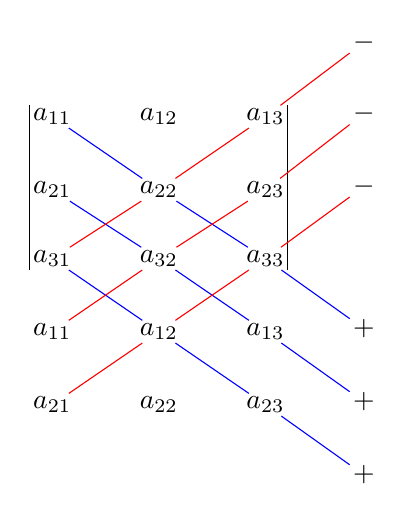
\begin{tikzpicture}
		\matrix (M) [matrix of math nodes , inner sep=1pt, row sep=0.6cm,column sep=8mm]{
			&&& -\\      
			a_{11} & a_{12} & a_{13} & - \\
			a_{21} & a_{22} & a_{23} & -\\ 
			a_{31} & a_{32} & a_{33} & \ \\
			a_{11} & a_{12} & a_{13} & + \\
			a_{21} & a_{22} & a_{23} & +\\
			&&& +\\  
		};
		
		
		\draw (M-2-1.north west) -- (M-4-1.south west) ;
		\draw (M-2-3.north east) -- (M-4-3.south east) ;
		
		\draw[blue](M-2-1)--(M-3-2)--(M-4-3)--(M-5-4);
		\draw[blue](M-3-1)--(M-4-2)--(M-5-3)--(M-6-4);
		\draw[blue](M-4-1)--(M-5-2)--(M-6-3)--(M-7-4);
		
		\draw[red](M-5-1)--(M-4-2)--(M-3-3)--(M-2-4);
		\draw[red](M-4-1)--(M-3-2)--(M-2-3)--(M-1-4);
		\draw[red](M-6-1)--(M-5-2)--(M-4-3)--(M-3-4);
	\end{tikzpicture}
\end{center}
o también:
\begin{center}
	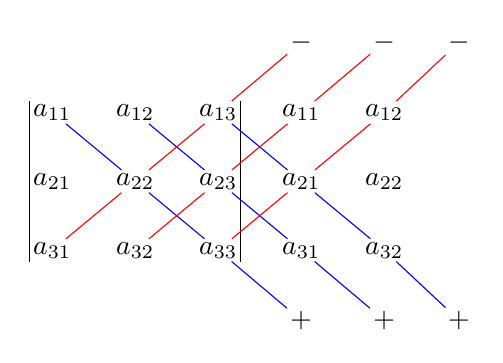
\begin{tikzpicture}
		\matrix (M) [matrix of math nodes , inner sep=1pt, row sep=0.6cm,column sep=5mm]{
			&&& - & - & -\\      
			a_{11} & a_{12} & a_{13} & a_{11} & a_{12} & \ \\
			a_{21} & a_{22} & a_{23} & a_{21} & a_{22} & \ \\ 
			a_{31} & a_{32} & a_{33} & a_{31} & a_{32} & \ \\
			&&& + & + & +\\  
		};
		
		\draw (M-2-1.north west) -- (M-4-1.south west) ;
		\draw (M-2-3.north east) -- (M-4-3.south east) ;
		
		\draw[blue](M-2-1)--(M-3-2)--(M-4-3)--(M-5-4);
		\draw[blue](M-2-2)--(M-3-3)--(M-4-4)--(M-5-5);
		\draw[blue](M-2-3)--(M-3-4)--(M-4-5)--(M-5-6);
		
		\draw[red](M-4-1)--(M-3-2)--(M-2-3)--(M-1-4);
		\draw[red](M-4-2)--(M-3-3)--(M-2-4)--(M-1-5);
		\draw[red](M-4-3)--(M-3-4)--(M-2-5)--(M-1-6);
	\end{tikzpicture}
\end{center}
Cabe resaltar que \textbf{este método es solo valido hasta una matriz de 3x3}.
\begin{Example*} {Método Sarrus para determinantes}
	Hallar el determinante de:
	$$
		A=\begin{bmatrix}
			1&3\\
			8&5
		\end{bmatrix}\text{ y } B=\begin{bmatrix}
			3&5&1\\
			0&-2&4\\
			1&-1&7
		\end{bmatrix}
	$$
	Sol:
	\begin{align*}
		|A|=&\begin{vmatrix}
				1&3\\
				8&5
			\end{vmatrix}\\
		=&(1)(5)-(8)(3)\\
		|A|=-19\\
		|B|=&\begin{array} {c}
			\begin{vmatrix}
				3&5&1\\
				0&-2&4\\
				1&-1&7
			\end{vmatrix}\\
			\begin{matrix}
				3&5&1\\
				0&-2&4
			\end{matrix}
		\end{array}\\
		=&(3)(-2)(7)+(0)(-1)(1)+(1)(5)(4)\\
		&-(1)(-2)(1)-(3)(-1)(4)-(0)(5)(7)\\
		|B|=-8
	\end{align*}
\end{Example*}
\subsubsection*{Método de operaciones elementales}
Este método consiste en transformar un determinante a una forma triangular superior o inferior, por medio de operaciones elementales y la propiedades de operaciones elementales-valores notables.
Un ventaja a diferencia del método Sarrus es que no importa el tamaño de la matriz.
\begin{align*}
	&\begin{array} {c}
		\begin{vmatrix}
			1&1&-2\\
			-1&2&1\\
			0&1&-1
		\end{vmatrix}\\
		f_1+f_2\rightarrow f_2
	\end{array}\begin{array} {c}
	=\begin{vmatrix}
		1&1&-2\\
		0&3&-1\\
		0&1&-1
	\end{vmatrix}\\
		1/3f_2\rightarrow f_2
	\end{array}	\begin{array} {c}
	=3\begin{vmatrix}
		1&1&-2\\
		0&1&-1/3\\
		0&1&-1
	\end{vmatrix}\\
		-f_1+f_3\rightarrow f_3
	\end{array}\\
	&3\begin{vmatrix}
		1&1&-2\\
		0&1&-1/3\\
		0&0&-2/3
	\end{vmatrix}=3\left(-\frac{2}{3}\right)=-2
\end{align*}
\subsection*{Menores y cofactores}
\subsubsection*{Menores}
Sea una matriz $n$-cuadrada $A=[a_{ij})$ y la submatriz $(n-1)$-cuadrada de A denotada por $M_{ij}$, que se obtine al suprimir $a_{ij}$, su $i$-ésima fila y su $j$-ésima columna. Entonces denominamos \textbf{menor} del elemento $a_{ij}$ de $A$ al determinante $|M_{ij}|$.
\begin{Example*} {Menores}
	Hallar el menor $|M_{11}|$, $|M_{22}|$ y $|M_{32}|$ de:
	$$ A=\begin{bmatrix}
		3&-1&2\\
		-1&9&3\\
		3&5&2
	\end{bmatrix} $$
	Sol. \\
	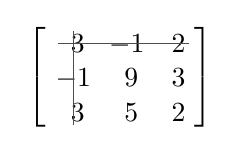
\begin{tikzpicture}
		\matrix (M) [matrix of math nodes , left delimiter={[},right delimiter={]} , inner sep=1pt, row sep=1.1mm,column sep=1.6mm]{    
			\ 3 & -1 & \ 2\\
			-1 & \ 9 & \ 3\\
			\ 3 & \ 5 & \ 2 \\
		};
		\draw [red] (M-1-1.north) -- (M-3-1.south) ;
		\draw [red] (M-1-1.west) -- (M-1-3.east) ;
	\end{tikzpicture}
	\begin{align*}
		&|M_{11}|=\begin{vmatrix}
			9&3\\
			5&2
		\end{vmatrix}=45-48=-3 \quad\quad\quad\quad
	\end{align*}
	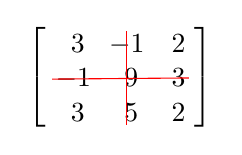
\begin{tikzpicture}
		\matrix (M) [matrix of math nodes , left delimiter={[},right delimiter={]} , inner sep=1pt, row sep=1.1mm,column sep=1.6mm]{    
			\ 3 & -1 & \ 2\\
			-1 & \ 9 & \ 3\\
			\ 3 & \ 5 & \ 2 \\
		};
		\draw [red] (M-1-2.north) -- (M-3-2.south) ;
		\draw [red] (M-2-1.west) -- (M-2-3.east) ;
	\end{tikzpicture}
	\begin{align*}
		&|M_{22}|=\begin{vmatrix}
			3&2\\
			3&2
		\end{vmatrix}=6-6=0 \quad\quad\quad\quad
	\end{align*}
	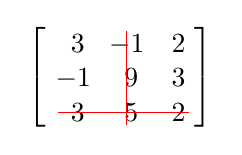
\begin{tikzpicture}
		\matrix (M) [matrix of math nodes , left delimiter={[},right delimiter={]} , inner sep=1pt, row sep=1.1mm,column sep=1.6mm]{    
			\ 3 & -1 & \ 2\\
			-1 & \ 9 & \ 3\\
			\ 3 & \ 5 & \ 2 \\
		};
		\draw [red] (M-1-2.north) -- (M-3-2.south) ;
		\draw [red] (M-3-1.west) -- (M-3-3.east) ;
	\end{tikzpicture}
	\begin{align*}
		&|M_{32}|=\begin{vmatrix}
			3&2\\
			-1&3
		\end{vmatrix}=9-(-2)=11 \quad\quad\quad\quad
	\end{align*}
\end{Example*}
Así también podemos hallar los menores de cada elemento de una matriz, y lo llamaremos matriz de menores.
\begin{Example*} {Matriz de menores}
	Hallar matriz de menores $M$ si:
	$$ A=\begin{bmatrix}
		9&0&-1\\
		3&5&2\\
		-7&3&1
	\end{bmatrix} $$
	Sol.
	\begin{align*}
		&A=\begin{bmatrix}
			9&0&-1\\
			3&5&2\\
			-7&3&1
		\end{bmatrix}\\
		&M=\begin{bmatrix}
			M_{11}&M_{12}&M_{13}\\
			M_{21}&M_{22}&M_{23}\\
			M_{31}&M_{32}&M_{33}
		\end{bmatrix}\\
		&M=\begin{bmatrix}
			\begin{vmatrix}
				5&2\\
				3&1
			\end{vmatrix}&\begin{vmatrix}
				3&2\\
				-7&1
			\end{vmatrix}&\begin{vmatrix}
				3&5\\
				-7&3
			\end{vmatrix}\\
			\begin{vmatrix}
				0&-1\\
				3&1
			\end{vmatrix}&\begin{vmatrix}
				9&-1\\
				-7&1
			\end{vmatrix}&\begin{vmatrix}
				9&0\\
				-7&3
			\end{vmatrix}\\
			\begin{vmatrix}
				0&-1\\
				5&2
			\end{vmatrix}&\begin{vmatrix}
				9&-1\\
				3&2
			\end{vmatrix}&\begin{vmatrix}
				9&0\\
				3&5
			\end{vmatrix}
		\end{bmatrix}\\
		&\therefore \ M=\begin{bmatrix}
			-1&17&44\\
			3&2&27\\
			5&21&45
		\end{bmatrix}
	\end{align*}
\end{Example*}
\subsubsection*{Cofactores}
Sea una matriz cuadrada $A=[a_{ij}]$ y $|M_{ij}|$ el menor del elemento $a_{ij}$; entonces definimos el cofactor de $a_{ij}$, denotado por $A_{ij}$ como el menor con signo:
$$ A_{ij}=(-1)^{i+j}|M_{ij} $$
Es decir si que si le colocamos a un menor el signo de acuerdo a $(-1)^{i+j}$, entonces ahora es un cofactor.
\begin{Example*} {Cofactor}
	Hallar el cofactor $A_{11}$, $A_{22}$ y $A_{32}$ si:
	$$ A=\begin{bmatrix}
		3&-1&2\\
		-1&9&3\\
		3&5&2
	\end{bmatrix} $$
	Sol. \\
	\begin{align*}
		&\text{si: } |M_{11}|=-3, \ |M_{22}|=0\text{ y }|M_{32}|=11\\
		&A_{11}=(-1)^{1+1}|M_{11}|\\
		&A_{11}=(-1)^2(-3)=-3\\
		&A_{22}=(-1)^{2+2}|M_{22}|\\
		&A_{22}=(-1)^4(0)=0\\
		&A_{32}=(-1)^{3+2}|M_{32}|\\
		&A_{32}=(-1)^5(11)=-11\\
	\end{align*}
\end{Example*}
Así también podemos hallar los cofactores de cada elemento de una matriz, y lo llamaremos matriz de cofactores. Sin embargo, note usted que los signos que acompañan a los menores se disponen en forma de tablero de ajedrez, con signos $+$ en la diagonal principal:
$$ \begin{bmatrix}
	+&-&+&-&\cdots\\
	-&+&-&+&\cdots\\
	+&-&+&-&\cdots\\
	-&+&-&+&\cdots\\
	\vdots&\vdots&\vdots&\vdots&\ddots\\
\end{bmatrix} $$
Esto resulta muy útil ya que no habrá la necesidad de hallar el signo del menor de la anterior manera.
\begin{Example*} {Matriz de cofactores}
	Hallar matriz de cofactores $C$ si:
	$$ A=\begin{bmatrix}
		9&0&-1\\
		3&5&2\\
		-7&3&1
	\end{bmatrix} \text{ y } M=\begin{bmatrix}
	-1&17&44\\
	3&2&27\\
	5&21&45
	\end{bmatrix} $$
	donde $M$ es la matriz de menores\\
	Sol.
	\begin{align*}
		&\text{si: } M=\begin{bmatrix}
			-1&17&44\\
			3&2&27\\
			5&21&45
		\end{bmatrix} \text{ y } \begin{bmatrix}
			+&-&+\\
			-&+&-\\
			+&-&+\\
		\end{bmatrix}\\
		&\therefore \ C=\begin{bmatrix}
			-1&-17&44\\
			-3&2&-27\\
			5&-21&45
		\end{bmatrix}
	\end{align*}
\end{Example*}

\subsection*{Matriz adjunta}
Sea una matriz $n$-cuadrada $A=[a_{ij}]$, su adjunta denotado por $\mathrm{adj}(A)$ es la traspuesta de la matriz de cofactores $C$ de $A$:
$$ \mathrm{Adj}(A)=C^T $$
\begin{Example*} {Matriz adjunta}
	Hallar la matriz adjunta de:
	$$ A=\begin{bmatrix}
		2&3&-4\\
		0&-4&2\\
		1&-1&5
	\end{bmatrix} $$
	Sol.
	\begin{flalign*}
		&A_{11}=+\begin{vmatrix}
			-4&2\\
			-1&5
		\end{vmatrix}=-18\\
		&A_{12}=-\begin{bmatrix}
			0&2\\1&5
		\end{bmatrix}=2\\
		&A_{13}=+\begin{bmatrix}
			0&-4\\
			1&-1
		\end{bmatrix}=4\\
		&A_{21}=-\begin{bmatrix}
			3&-4\\
			-1&5
		\end{bmatrix}=-11\\
		&A_{22}=+\begin{bmatrix}
			2&-4\\
			1&5
		\end{bmatrix}=14\\
		&A_{23}=-\begin{bmatrix}
			2&3\\
			1&-1
		\end{bmatrix}=5\\
		&A_{31}=+\begin{bmatrix}
			3&-4\\
			-4&2
		\end{bmatrix}=-10\\
		&A_{32}=-\begin{bmatrix}
			2&-4\\
			0&2
		\end{bmatrix}=-4\\
		&A_{33}=+\begin{bmatrix}
			2&3\\
			0&-4
		\end{bmatrix}=-8\\
		&C=\begin{bmatrix}
			-18&2&4\\
			-11&14&5\\
			-10&-4&-8
		\end{bmatrix}\\
		&\Rightarrow C^T=\begin{bmatrix}
			-18&-11&-10\\
			2&14&-4\\
			4&5&-8
		\end{bmatrix}\\
		&\therefore \ \mathrm{Adj}(A)=\begin{bmatrix}
			-18&-11&-10\\
			2&14&-4\\
			4&5&-8
		\end{bmatrix}
	\end{flalign*}
\end{Example*}
\subsubsection*{Propiedades de la matriz adjunta}
Sean $A$,$B$ e $I$ matrices $n$-cuadradas, donde $I$ es la matriz identidad, ademas $k$ y $n$ son constante, entonces:
\begin{enumerate}
	\item $ \mathrm{Adj}(I)=I $
	\item $ \mathrm{Adj}(A^k)=[\mathrm{Adj}(A)]^k $
	\item $ \mathrm{Adj}(AB)=\mathrm{Adj}(B)\mathrm{Adj}(A) $
	\item $ |\mathrm{Adj}(A)|=|A|^{n-1}$
	\item $ |\mathrm{Adj}(kA)|=k^{n(n-1)}|A|^{n-1} $
	\item $ \mathrm{Adj}(A^T)=[\mathrm{Adj}(A)]^T $
\end{enumerate}
\subsection*{Calculo de determinantes II}
\subsubsection*{Metodo de cofactores}
Sea una matriz cuadrada $A=[a_{ij}]$ entonces su determinante es la sumatoria al producto parcial de los elementos de una fila o columna cualquiera por sus correspondientes cofactores.
$$ \det(A)=\sum_{k=1}^{n}a_{ik}C_{ik} \longrightarrow \text{ (para filas) } $$
$$ \det(A)=\sum_{k=1}^{n}a_{kj}C_{kj} \longrightarrow \text{ (para columnas) } $$
Es decir, este método consiste en elegir una fila o columna cualquiera, el cual se suma el producto de elemento por el cofacator de cada elemento.
\begin{Example*} {Método de cofactores - ejemplo 1}
	Hallar la determinante de:
	$$ A=\begin{bmatrix}
		3&5&-1\\
		2&-3&6\\
		7&0&4
	\end{bmatrix} $$
	Sol.\\
	Seleccionar una fila o columna
	\begin{center}
		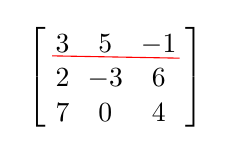
\begin{tikzpicture}
			\matrix (M) [matrix of math nodes , left delimiter={[},right delimiter={]} , inner sep=1pt, row sep=1.1mm,column sep=1.6mm]{    
				3 & 5 & -1\\
				2 & -3 & 6\\
				7 & 0 & 4\\
			};
			\draw [red] (M-1-1.south west) -- (M-1-3.south east);
		\end{tikzpicture}
	\end{center}
	hallamos sus cofactores
	\begin{center}
		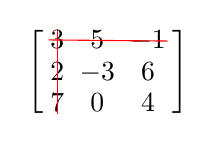
\begin{tikzpicture}
			\matrix (M) [matrix of math nodes , left delimiter={[},right delimiter={]} , inner sep=0.5pt, row sep=1.1mm,column sep=1.6mm]{    
				3 & 5 & -1\\
				2 & -3 & 6\\
				7 & 0 & 4\\
			};
			\draw [red] (M-1-1.north) -- (M-3-1.south);
			\draw [red] (M-1-1.west) -- (M-1-3.east);
		\end{tikzpicture}
		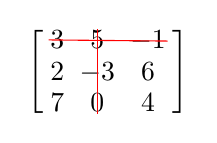
\begin{tikzpicture}
			\matrix (M) [matrix of math nodes , left delimiter={[},right delimiter={]} , inner sep=0.5pt, row sep=1.1mm,column sep=1.6mm]{    
				3 & 5 & -1\\
				2 & -3 & 6\\
				7 & 0 & 4\\
			};
			\draw [red] (M-1-2.north) -- (M-3-2.south);
			\draw [red] (M-1-1.west) -- (M-1-3.east);
		\end{tikzpicture}
		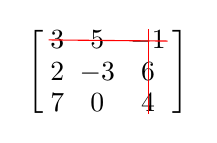
\begin{tikzpicture}
			\matrix (M) [matrix of math nodes , left delimiter={[},right delimiter={]} , inner sep=0.5pt, row sep=1.1mm,column sep=1.6mm]{    
				3 & 5 & -1\\
				2 & -3 & 6\\
				7 & 0 & 4\\
			};
			\draw [red] (M-1-3.north) -- (M-3-3.south);
			\draw [red] (M-1-1.west) -- (M-1-3.east);
		\end{tikzpicture}
	\end{center}
	\begin{align*}
		&A_{11}=-12 \quad\quad A_{12}=-34 \quad\quad A_{13}=21
		\intertext{hallamos su determinante}
		&|A|=\begin{vmatrix}
			3&5&-1\\
			2&-3&6\\
			7&0&4
		\end{vmatrix}\\
		&=a_{11}(-1)^2A_{11}+a_{12}(-1)^3A_{12}+a_{13}(-1)^4A_{13}\\
		&=(3)(-12)+(5)(-1)(-34)+(-1)(21)\\
		&=113\\
		&\therefore \ |A|=113
	\end{align*}
\end{Example*}
Este metodo es mas util para matrices con fila o columnas que tengas elementos nulos (ceros) ya que al multiplicar por elemento esta se anula:
\begin{Example*} {Metodo de cofactores - ejemplo 2}
	Hallar la determinante de:
	$$ A=\begin{bmatrix}
		0&0&-2&3&1&2\\
		1&-1&2&-1&0&-3\\
		3&0&1&-1&-2&4\\
		5&0&-4&3&1&1\\
		-2&0&2&9&-9&1\\
		8&0&-3&1&-1&0
	\end{bmatrix} $$
	Sol.
	\begin{align*}
		|A|=(-1)\begin{vmatrix}
			0&-2&3&1&2\\
			3&1&-1&-2&4\\
			5&-4&3&1&1\\
			-2&2&9&-9&1\\
			8&-3&1&-1&0
		\end{vmatrix}
	\end{align*}
\end{Example*}
\subsubsection*{Método de Chio (Método combinado)}
Este método consiste en transformar por medio de operaciones elementales una determinante con el objetivo de generar ceros en fila o columna, una ves esto por el método de cofactores encontrar la determinante.
\begin{Example*} {Metodo de Chio}
	Hallar el determinante de:
	$$ A=\begin{bmatrix}
		1&234/134&\sqrt{249}\\
		-1&2&1\\
		0&1&-1
	\end{bmatrix} $$
	Sol.
	\begin{align*}
		&\begin{matrix}
			|A|=\begin{vmatrix}
				1&\frac{234}{134}&\sqrt{349}\\
				-1&2&1\\
				0&1&-1
			\end{vmatrix}\\
			f_1+f_2\rightarrow f_2
		\end{matrix} \begin{matrix}
			=\begin{vmatrix}
				1&\frac{234}{134}&\sqrt{349}\\
				0&3&-1\\
				0&1&-1
			\end{vmatrix}\\
			\
		\end{matrix}\\
		&|A|=(1)\begin{vmatrix}
			3&-1\\
			1&-1
		\end{vmatrix}-\cancel{(0)\begin{vmatrix}
			\frac{234}{134}&\sqrt{349}\\
			1&-1
		\end{vmatrix}}\\
		&\quad\quad+\cancel{(0)\begin{vmatrix}
			\frac{234}{134}&\sqrt{349}\\
			3&-1
		\end{vmatrix}}\\
		&|A|=\begin{vmatrix}
			3&-1\\
			1&-1
		\end{vmatrix}=3(-1)-(1)(-1)=-2
	\end{align*}
\end{Example*}
\subsection*{Matriz inversa II}
Recordemos que una matriz inversa es aquella que cumple lo siguiente:
$$ AB=BA=I \Rightarrow B=A^{-1} $$
donde $A$ y $B$ son matrices cuadradas, y $B$ viene siendo la matriz inversa de $A$; es decir:
$$ AA^{-1}=A^{-1}A=I $$
No toda matriz es invertible. Una matriz cuya determinada es nulo, no tiene su inversa, a esto se denomina matriz singular:
$$ |A|=0 \Rightarrow \nexists A^{-1} \text{ (matriz singular)} $$
$$ |A|\ne0 \Rightarrow \exists A^{-1} \text{ (matriz invertible)} $$
\subsubsection*{Propiedades de la matriz inversa}
\begin{enumerate}
	\item $ A\emptyset=\emptyset A=\emptyset $
	\item $ AB=\emptyset \Rightarrow B=\emptyset $
	\item $ (A^{-1})^{-1}=A $
	\item $ (AB)^{-1}=B^{-1}A^{-1} $
	\item $ (kA)^{-1}=k^{-1}A^{-1} $
	\item $ I^{-1}=I $
	\item $ (A^T)^{-1}=(A-1)^T $
	\item $ (A^n)^{-1}=(A^{-1})^n $
	\item $ \mathrm{Adj}(A^{-1})=|A^{-1}|(A^{-1})^{-1} $
	\item $ \mathrm{Adj}(A^{-1})=\frac{1}{|A|}A=\frac{A}{|A|} $
\end{enumerate}
\subsubsection*{Método de la adjunta}
Para toda matriz cuadrada $A$, se cumple que:
$$ A\cdot\mathrm{Adj}(A)=\mathrm{Adj}(A)\cdot=|A|I $$
donde $I$ es la matriz identidad, y $|A|\ne 0$, entonces:
$$ A^{-1}=\frac{1}{|A|}\mathrm{Adj(A)} $$
\subsubsection*{Método por operaciones elementales (Gauss-Jordan)}
Este metodo ya lo usamos cuando vimos por primera vez matrices inversas. Esta consiste en transforma dos matrices simultaneamente: $A$ e $I$ donde $A$ es la matriz que queremos invertir e $I$ es la matriz identidad; debemos trasformar $A$ en una matriz identidad, una vez realizado esto $I$ se habra transformado en $A^{-1}$, es decir:
$$ [A|I]\xrightarrow[\text{operaciones elementales}]{\text{transformar con}}[I|A^{-1}] $$
		\setcounter{exr}{0} 
		\end{multicols}
\section{Sistema de ecuaciones lineales}
\subsubsection*{Ecuaciones lineales}
Una ecuación lineal en las variables $ x_1, x_2, x_3,\dots , x_n $ tiene la forma:
$$ a_1x_1+a_2x_2+a_3x_3+\dots+a_nx_n=b_1 $$
donde: $ a_1,a_2,a_3,\dots,a_n,b_1 \in \mathbb{R} $. \\
por ejemplo
\begin{flalign*}
	&\begin{array} {l}
		2x+9y-3z=2\longrightarrow \text{(es ecuación lineal)}\\
		x_1-2x_2=0\longrightarrow \text{(es ecuación lineal)}\\
		x_1+x_2+\dots+x_n=1\longrightarrow \text{(es ecuación lineal)}\\
	\end{array} &\begin{array} {l}
		3xy-2y=9\longrightarrow \text{(no es ecuación lineal)}\\
		9y^2-\frac{2}{x}=-2\longrightarrow \text{(no es ecuación lineal)}\\
		x^2y-1=y\longrightarrow \text{(no es ecuación lineal)}\\
	\end{array}
\end{flalign*}
\subsubsection*{Sistema de ecuaciones lineales}
Es un conjunto finito de ecuaciones lineales
$$ \left\{\begin{matrix}
	a_{11}x_1+a_{12}x_2+a_{13}x_3+\dots+ \ a_{1n}x_n=b_1\\
	a_{21}x_1+a_{22}x_2+a_{23}x_3+\dots+ \ a_{2n}x_n=b_2\\
	a_{31}x_1+a_{32}x_2+a_{33}x_3+\dots+ \ a_{3n}x_n=b_3\\
	\vdots\\
	a_{m1}x_1+a_{m2}x_2+a_{m3}x_3+\dots+a_{mn}x_n=b_m\\
\end{matrix}\right. $$
En función a la definición de igualdad de matrices, es decir dos matrices son iguales cuando tienen el mismo tamaño y sus elementos son iguales posición a posición, entonces podemos pasar de un sistema de ecuaciones a una matricial:
$$
	\begin{bmatrix}
		a_{11}x_1+a_{12}x_2+a_{13}x_3+\dots+ \ a_{1n}x_n\\
		a_{21}x_1+a_{22}x_2+a_{23}x_3+\dots+ \ a_{2n}x_n\\
		a_{31}x_1+a_{32}x_2+a_{33}x_3+\dots+ \ a_{3n}x_n\\
		\vdots\\
		a_{m1}x_1+a_{m2}x_2+a_{m3}x_3+\dots+a_{mn}x_n\\
	\end{bmatrix}_{m\cross 1}=\begin{bmatrix}
		b_1\\
		b_2\\
		b_3\\
		\vdots\\
		b_m
	\end{bmatrix}_{m\cross 1}
$$
Ahora podemos separar los coeficientes de sus variables con el producto de matrices:
$$
	\begin{bmatrix}
		a_{11}&a_{12}&a_{13}&\cdots&a_{1n}\\
		a_{21}&a_{22}&a_{23}&\cdots&a_{2n}\\
		a_{31}&a_{32}&a_{33}&\cdots&a_{3n}\\
		\vdots&\vdots&\vdots&\ddots&\vdots\\
		a_{m1}&a_{m2}&a_{m3}&\cdots&a_{mn}\\
	\end{bmatrix}_{m\cross n}\begin{bmatrix}
		x_1\\
		x_2\\
		x_3\\
		\vdots\\
		x_n
	\end{bmatrix}_{n\cross 1}=\begin{bmatrix}
		a_{11}x_1+a_{12}x_2+a_{13}x_3+\dots+ \ a_{1n}x_n\\
		a_{21}x_1+a_{22}x_2+a_{23}x_3+\dots+ \ a_{2n}x_n\\
		a_{31}x_1+a_{32}x_2+a_{33}x_3+\dots+ \ a_{3n}x_n\\
		\vdots\\
		a_{m1}x_1+a_{m2}x_2+a_{m3}x_3+\dots+a_{mn}x_n\\
	\end{bmatrix}_{m\cross 1}
$$
Entonces
$$
	\begin{bmatrix}
		a_{11}&a_{12}&a_{13}&\cdots&a_{1n}\\
		a_{21}&a_{22}&a_{23}&\cdots&a_{2n}\\
		a_{31}&a_{32}&a_{33}&\cdots&a_{3n}\\
		\vdots&\vdots&\vdots&\ddots&\vdots\\
		a_{m1}&a_{m2}&a_{m3}&\cdots&a_{mn}\\
	\end{bmatrix}_{m\cross n}\begin{bmatrix}
		x_1\\
		x_2\\
		x_3\\
		\vdots\\
		x_n
	\end{bmatrix}_{n\cross 1}=\begin{bmatrix}
		b_1\\
		b_2\\
		b_3\\
		\vdots\\
		b_m
	\end{bmatrix}_{m\cross 1}
$$
finalmente obtenemos un sistema matricial de ecuaciones lineales, donde podemos trabajar, transforma y el cual es nuestro objetivo resolver el sistema, usando distintos propiedades matriciales que ya aprendimos:
$$ A_{m\cross n}X_{n\cross 1} = B_{m\cross 1} $$
por lo tanto:
\begin{Theorem*} {Teoría del álgebra lineal para resolución de sistema de ecuaciones lineales}
	Sea sistema de ecuaciones lineales de la forma:
	$$ a_1x_1+a_2x_2+a_3x_3+\dots+a_nx_n=b_1 $$
	se puede expresar a una forma de de ecuación matricial:
	$$ A_{m\cross n}X_{n\cross 1} = B_{m\cross 1} $$
	donde $A$ es la matriz de coeficientes que pertenecen a $\mathbb{R}$, $X$ es la matriz de variables y $B$ es la matriz de términos independientes que pertenecen a $\mathbb{R}$.
\end{Theorem*}
\subsection*{Tipos de soluciones}
\subsection*{Métodos de resolución}
\subsubsection*{Método de la inversa}
\begin{Theorem*} {Metodo de la inversa}
	Sea $A$ una \textbf{matriz $n$-cuadrada}, $B$ matriz de terminos independientes y $X$ es la matriz de variables, entonces:
	\begin{gather*}
		AX=B\\
		A^{-1}AX=A^{-1}B
	\end{gather*}
	donde:
	$$ A_{n\cross n}, |A|\ne 0, A=[a_{ij}] \in \mathbb{R}, B=[b_{ij}] \in \mathbb{R} $$
	por lo tanto:
	$$ X=A^{-1}B $$
\end{Theorem*}
\subsubsection*{Método de Gauss o forma escalonada}
\begin{Theorem*} {Método de Gauss}
	Sea $A$,$B$y$X$ la matriz de coeficientes, terminos independientes y de variables respectivamente; $U$ una matriz triangular superior y $B'$ una matriz transformada por operaciones elementales a partir de $B$. Entonces:
	\begin{gather*}
		AX=B\\
		[A|B]\xrightarrow[\text{operaciones elementales}]{\text{Transformar por}}[U|B']\\
		UX=B'
	\end{gather*}
	donde:
	$$ A=[a_{ij}] \in \mathbb{R}, B=[b_{ij}] \in \mathbb{R} $$
\end{Theorem*}
\subsubsection*{Método de Gauss-Jordan o forma escalonada reducida}
\begin{Theorem*} {Método de Gauss-Jordan}
	Sea $A$,$B$y$X$ la matriz de coeficientes, terminos independientes y de variables respectivamente; $I$ e $I'$ una matriz identidad y matriz semejante a la identidad; y $B'$ una matriz transformada por operaciones elementales a partir de $B$. Entonces:
	$$ AX=B $$
	existen dos casos:
	\begin{enumerate}
		\item se llega a la matriz identidad $I$:
		\begin{gather*}
			[A|B]\xrightarrow[\text{operaciones elementales}]{\text{Transformar por}}[I|B']\\
			IX=B'
		\end{gather*}
		\item se llega a una matriz $I'$ parecida a la identidad, debido a que $A$ no es invertible:
		\begin{gather*}
			[A|B]\xrightarrow[\text{operaciones elementales}]{\text{Transformar por}}[I'|B']\\
			I'X=B'
		\end{gather*}
	\end{enumerate}
	donde:
	$$ A=[a_{ij}] \in \mathbb{R}, B=[b_{ij}] \in \mathbb{R} $$
\end{Theorem*}
\subsubsection*{Metodo Cramer}
\begin{multicols}{2}
		\setcounter{exr}{0} 
		\section{Espacios vectoriales, combinaciones lineales, bases y dimensiones}
\subsection*{Espacios vectoriales}
La definicion de espacio vectorial involucra un cuerpo arbitrario cuyos elementos se denominan \textit{escalares}, se utilizaran los siguiente notacion:
\begin{flalign*}
	K&\quad \text{el cuerpo de escalares}\\
	a, b, c \text{ o } k&\quad \text{los elemento de K}\\
	V&\quad \text{el espacio vectorial dado}\\
	\vec{u},\vec{v},\vec{w}&\quad \text{los elementos de }V\\
	\vec{\phi}&\quad\text{vector nulo (vació)}
\end{flalign*}
\begin{Theorem*} {Definición - Espacios vectoriales}
	Sea $K$ un cuerpo dado y $V$ un conjunto no vacio, con reglas de suma y producto por un escalar que asignan a ada par $u$, $v$ $\in V$ una \textbf{suma} $u + v \in V$  a cada par $u\in V$, $k\in K$ un \textbf{producto} $ku\in V$. $V$ recibe el nombre de \textbf{espacio vectorial} sobre $K$ (y los elementos de $V$ se llaman vectores) si se satisfacen 5 axiomas para la suma y 5 axiomas para el producto por un escalar.
\end{Theorem*}
Por lo tanto, un espacio vectorial es un conjunto de vectores-escalares que cumplen la estructura: 
$$ (V,+,\cdot) $$
es decir, que satisfacen los siguientes axiomas:\\\\
\textbf{\textit{5 axiomas para la suma de vectores}}
\begin{enumerate}
	\item Clausura para la suma:
	$$ \vec{u}+\vec{v}\in V $$
	\item Conmutabilidad para la suma:
	$$ \vec{u}+\vec{v}=\vec{v}+\vec{u} $$
	\item Asociatividad para la suma:
	$$ (\vec{u}+\vec{v})+\vec{w}=\vec{u}+(\vec{v}+\vec{w}) $$
	\item Existencia del neutro aditivo:
	$$ \vec{u}+\vec{\phi}=\vec{u} $$
	\item Existencia del inverso aditivo:
	$$ \vec{u}+\vec{u}'=\vec{\phi} \quad\quad \text{es decir: } \vec{u}+(-\vec{u})=\vec{\phi} $$
\end{enumerate}
\textbf{\textit{5 axiomas para el producto por un escalar}}
\begin{enumerate}
	\setcounter{enumi}{5}
	\item Clausura para el producto por un escalar:
	$$ k\vec{u}\in V $$
	\item Asociatividad del producto por un escalar
	$$ (ab)\vec{u}=a(b\vec{u}) $$
	\item $1^{ra}$propiedad distributiva referida a la suma de escalares:
	$$ (a+b)\vec{u}=a\vec{u}+b\vec{u} $$
	\item $2^{da}$propiedad distributiva referida a la suma de vectores:
	$$ k(\vec{u}+\vec{v})=k\vec{u}+k\vec{v} $$
	\item Existencia del neutro multiplicativo:
	$$ k\vec{u}=\vec{u}\quad\quad k=1 $$
\end{enumerate}
\end{multicols}
\subsection*{Ejemplos de espacios vectoriales}
\subsubsection*{Espacio $K$}
\subsubsection*{Espacio de matrices $M_{m\cross n}$}
\subsubsection*{Espacio de polinomios $P(t)$}
Denotamos por P(t) el conjunto de todos los polinomios
\begin{Example*} {Espacio de funciones - ej 1}
	Analizar si las funciones de la forma $k_1+k_2\sen(x)$ donde $k_1, k_2, \in \mathbb{R}$, constituyen un espacio vectorial.
	Sol.
	\begin{align*}
		f(x)=k_1+k_2\sen(x)\\
		g(x)=k_3+k_4\sen(x)\\
		h(x)=k_5+k_6\sen(x)
	\end{align*}
	\begin{align*}
		\intertext{i) clausura para la suma}
		&\vec{u}+\vec{v}\in V\\
		f(x)+g(x)&=[k_1+k_2\sen(x)]+[k_1+k_2\sen(x)]\\
		&=k_1+k_2\sen(x)+k_3+k_4\sen(x)\\
		&=(k_1+k_3)+(k_2+k_4)\sen(x)\\
		&=k_a+k_b\sen(x) \Longrightarrow \text{(cumple)}
		\intertext{ii) conmutabilidad para la suma}
		&\vec{u}+\vec{v}=\vec{v}+\vec{u}\\
		f(x)+g(x)&=[k_1+k_2\sen(x)]+[k_1+k_2\sen(x)]\\
		&=k_1+k_2\sen(x)+k_3+k_4\sen(x)\\
		&=(k_3+k_4\sen(x))+(k_1+k_2\sen(x))\\
		&=g(x)+f(x)\Longrightarrow\text{(cumple)}
		\intertext{iii) Asociatividad en la suma}
		&(\vec{u}+\vec{v})+\vec{w}=\vec{u}+(\vec{v}+\vec{w})\\
		[f(x)+g(x)]+h(x)&=[k_1+k_2\sen(x)+k_3+k_4\sen(x)]+k_5+k_5\sen(x)\\
		&=k_1+k_2\sen(x)+k_3+k_4\sen(x)+k_5+k_6\sen(x)\\
		&=k_1+k_2\sen(x)+[k_3+k_4\sen(x)+k_5+k_6\sen(x)]\\
		&=f(x)+[g(x)+h(x)]\Longrightarrow \text{(cumple)}
		\intertext{iv) Existencia del neutro aditivo}
		&\vec{u}+\vec{\phi}=\vec{u}\\
		f(x)+\phi(x)&=f(x)\\
		k_1+k_2\sen(x)\phi(x)&=k_1+k_2\sen(x)\\
		\phi(x)&=(k_1-k_1)+(k_2-k_2)\sen(x)\\
		\phi(x)&=0+0\sen(x)\Longrightarrow\text{(cumple)}
		\intertext{v) Existencia del inverso aditivo}
		&\vec{u}+\vec{u}^-=\vec{\phi}\\
		f(x)+f(x)^-&=\phi(x)\\
		k_1+k_2\sen(x)+f(x)^-=&0+0\sen(x)\\
		f(x)^-&=(0-k_1)+(0-k_2)\sen(x)\\
		f(x)^-&=(-k_1)+(-k_2)\sen(x)\Longrightarrow\text{(cumple)}
		\intertext{vi) clausura para el producto por un escalar}
		&k\vec{u}\in V\\
		kf(x)&=k(k_1+k_2\sen(x))\\
		&=kk_1+kk_2\sen(x)\\
		&=k_c+k_d\sen(x)\Longrightarrow\text{(cumple)}
		\intertext{vii) Asocitividad para el producto por un escalar}
		&(ab)\vec{u}=a(b\vec{u})\\
		(ab)f(x)&=(ab)(x_1+x_2\sen(x)\\
		&=abx_1+abx_2\sen(x)\\
		&=a(bx_1+bx_2\sen(x))\\
		&=a(b(x_1+x_2\sec(x)))\\
		&=a(bf(x))\Longrightarrow\text{(cumple)}
		\intertext{viii) 1ra prop. distributiva referida a la suma de escalares}
		&(a+b)\vec{u}=a\vec{u}+b\vec{u}\\
		(a+b)f(x)&=(a+b)(x_1+x_2\sen(x))\\
		&=(a+b)x_1+(a+b)x_2\sen(x)\\
		&=ax_1+bx_1+ax_2\sen(x)+bx_2\sen(x)\\
		&=ax_1+ax_2\sen(x)+bx_1+bx_2\sen(x)\\
		&=a(x_1+x_2\sen(x))+b(x_1+x_2\sen(x))\\
		&=af(x)+bf(x)\Longrightarrow\text{(cumple)}
		\intertext{ix) 2da prop distributiva referida a la suma de vectores}
		&k(\vec{u}+\vec{v})=k\vec{u}+k\vec{v}\\
		k(f(x)+g(x))&=k[(k_1+k_3)+(k_2+k_4)\sen(x)]\\
		&=k(k_1+k_3)+k(k_2+k_4)\sen(x)\\
		&=kk_1+kk_3+kk_2\sen(x)+kk_4\sen(x)\\
		&=[kk_1+kk_2\sen(x)]+[kk_3+kk_4\sen(x)]\\
		&=k(k_1+k_2\sen(x))+k(k_3+k_4\sen(x))\\
		&=kf(x)+kg(x)\Longrightarrow\text{(cumple)}\\
		\intertext{x) Existencia del neutro multiplicativo}
		&k\vec{u}=\vec{u}\\
		&kf(x)=f(x)\\
		&k(k_1+k_2\sen(x))=k_1+k_2\sen(x)\\
		&kk_1+kk_2\sen(x)=k_1+k_2\sen(x)\\
		&kk_1=k\rightarrow k=\frac{k_1}{k_2}=1\\
		&kk_2\sen(x)=k_2\sen(x)\rightarrow k=1\\
		&1f(x)=k_1+k_2\sen(x)\Longrightarrow\text{(cumple)}
	\end{align*}
\end{Example*}
\subsubsection*{Espacios de funciones}
\begin{multicols}{2}
\subsection*{Subespacio vectorial}
\begin{Theorem*} {Subespacio vectorial}
	Sea $W$ un subconjunto de un espacio vectorial $V$ sobre un cuerpo $K$. $W$ se denomina un subespacio de $V$ si es a su vez un espacio vectorial sobre $K$ con respecto a las operaciones de $V$, suma vectorial y producoto por un esacalar. 
\end{Theorem*}
Es decir, es un subconjunto del conjunto $V$ (espacio vectorial), el cual cumple 2 axiomas de clausura para la suma y para el producto por un escalar:
\begin{enumerate}
	\item Clausura para la suma:
	$$ \vec{u}+\vec{v}\in V $$
	\item Clausura para el producto por un escalar:
	$$ k\vec{u}\in V $$
\end{enumerate}
\noindent en otras palabras es como un resumen del espacio vectorial.
\begin{Example*} {Subespacio vectorial - ejemplo 1}
	Demostrar que el conjunto $W={(x,y)\in\mathbb{R}^2/y=10x}$ es un subespacio de $\mathbb{R}^2$.
	Sol.
	\begin{align*}
		&\vec{u}_1=(x_1,y_1)\in W\leftrightarrow y_1=10x_1\\
		&\vec{u}_2=(x_2,y_2)\in W\leftrightarrow y_2=10x_2\\
		&\text{clausura para la suma}\\
		&\vec{u}_1+\vec{u}_2=(x_1,y_1)+(x_2+y_2)\\
		&=(x_1+x_2,y_1+y_2)\\
		&=(x_1+x_2,10x_1+10x_2)\\
		&=((x_1+x_2),10(x_1,x_2))\\
		&=(x_a,10(x_a))\\
		&=(x_1,y_a)\in W\Longrightarrow\text{(cumple)}\\
		&\text{clausura para el producto}\\
		&k\vec{u}=k(x_1,y_1)\\
		&=(kx_1,ky_1)\\
		&=(kx_1,k(10x_1))\\
		&=(kx_1,10kx_1)\in W \Longrightarrow\text{(cumple)}\\
		&\therefore W \text{ es un subespacio vectorial}
	\end{align*}
\end{Example*}
\begin{Example*} {Subespacio vectorial - ejemplo 2}
	Dado el conjunto $W={(a,b,c)\in \mathbb{R}/a+b-c+3=k}$. Hallar "$k$" para que $W$ sea subespacio vectorial.
	Sol.
	\begin{align*}
		&\vec{u}_1=(a_1,b_1,c_1)\leftrightarrow a_1+b_1-c_1+3=k\\
		&\vec{u}_2=(a_2,b_2,c_2)\leftrightarrow a_2+b_2-c_2+3=k\\
		&\text{clausura para la suma}\\
		&\vec{u}_1+\vec{u}_2=(a_1,b_1,c_1)+(a_2,b_2,c_2)\\
		&=(a_1+a_2,b_1+b_2,c_1+c_2)\in W\\
		&(a_1+a_2)+(b_1+b_2)-(c_1+c_2)+3=k\\
		&\underbrace{(a_1+b_1-c_1)}_{k-3}+\underbrace{(a_2+b_2-c_2)}_{k-3}+3=k\\
		&k-3+k-3+3=k\rightarrow k=3\\
		&\text{clausura para el producto}\\
		&\alpha\vec{u}_1=\alpha(a_1,b_1,c_1)=(\alpha a_1,\alpha b_1, \alpha c_1)\\
		&\alpha a_1+\alpha b_1 - \alpha c_1+3=k\\
		&\alpha\underbrace{(a_1+b_1-c_1)}_{k-3}+3=l\\
		&\alpha(k-3)+3=k\\
		&\alpha(k-3)-(k-3)=0\\
		&(k-3)(\alpha-1)=0\Rightarrow k=3 \text{ y } \alpha=1\\	
	\end{align*}
	$\therefore$ Para $k=3$, $W$ es un subespacio vectorial
\end{Example*}
\begin{Example*} {Subespacio vecotorial - ejemplo 3}
	Analizar si el conjunto $S={(x,y)\in \mathbb{R}^2/y\ge 0}$ constituye o no un subespacio vectorial.
	\begin{gather*}
		\vec{a}=(x,y)\in\mathbb{R}\leftrightarrow y\ge0\\
		\vec{b}=(z,w)\in\mathbb{R}\leftrightarrow x\ge0
	\end{gather*}
	Sol.
	\begin{align*}
		&\text{clausura para la suma}\\
		&\vec{a}+\vec{b}=(x,y)+(z,w)\\
		&=(x+z,y+w)\\
		&=(k_1,k_2)\Rightarrow k_2\ge 0\Longrightarrow\text{(cumple)}\\
		&\text{clausura para el producto por escalar}\\
		&k\vec{a}=k(x,y)=(kx,ky)\\
		&ky=\left\{\begin{array}{llr}
			i) k (-) &  ky<0 & \text{(no cumple)}\\
			ii) k (+) & ky\ge 0 & \text{(cumple)}
		\end{array}\right.\\
		&\therefore S \text{ no es un subespacio vectorial}
	\end{align*}
\end{Example*}
\begin{Example*} {Subespacio vectorial - ejemplo 4}
	Sea $V$ un espacio vectorial de matrices $2\cross2$ sobre $\mathbb{R}$ y $W$ consta de todas las matrices tal que $A^2=A$. Determinar si $W$ es un subespacio vectorial de $V$.
	Sol.
	\begin{align*}
		&W={A\in\mathbb{R}^{2\cross2}/A^2=A}\\
		&A_1\leftrightarrow A_1^2=A_1\\
		&A_2\leftrightarrow A_2^2=A_2\\
		&\text{clausura para la suma}\\
		&A_1+A_2=(A_1+A_2)^2=(A_1+A_2)(A_1+A_2)\\
		&=A_1^2+2A_1A_2+A_2^2\\
		&\Rightarrow A_1+A_2\ne (A_1+A_2)^2\Longrightarrow\text{(no cumple)}\\
		&\therefore W \text{ no es un subespacio vectorial}
	\end{align*}
\end{Example*}
\subsection*{Combinaciones lineales}
La combinacion lineal es un concepto que se ha visto  anteriormente, como en fisica basica, por ejemplo:
sea el vector $a=$
\begin{figure}[H]
	\centering
	\begin{tikzpicture}[scale=1.2]
		\begin{axis}[xmin=-5,xmax=5,ymin=-1,ymax=7,axis x line=center, axis y line=center, yticklabel=\empty, xticklabel=\empty, xlabel=$x$, ylabel=$y$, xlabel style={at={(ticklabel* cs:1.05)}}, ylabel style={at={(ticklabel* cs:1.05)}}]
			\addplot [color=red!80,thick,samples=200]{4};
			\node at (axis cs:3,4.5) {$f(x)=b$};
		\end{axis}
	\end{tikzpicture}
\end{figure}
Sea $V$ un espacio vectoriales, $\vec{x}=(x_1,x_2,x_3,\dots,x_n)$ un elemento de dicho conjunto y un subconjunto $W={\vec{y},\vec{z},\dots,\vec{w}}$. Entonces $\vec{x}$ es combinacion lineal de $W$ si se comprueba:
$$ \vec{x}=a_1\vec{y}+a_2\vec{z}+\dots+a_3\vec{w} $$
\begin{Example*} {Combinacion lineal - ejemplo 1}
	En $\mathbb{R}^3$, escribir $\vec{x}=(1,2,3)$ como combinacion lineal de $\vec{u}=(1,0,1)$ $\vec{v}=(2,-1,1)$ y $\vec{w}=(1,1,1)$
	Sol.
	\begin{align*}
		&\vec{x}=\alpha\vec{u}+\beta\vec{v}+\gamma\vec{w}\\
		&(1,2,3)=\alpha(1,0,1)+\beta(2,-1,1)+\gamma(1,1,1)\\
		&(1,2,3)=(\alpha,0,\alpha)+(2\beta,-\beta,\beta)+(\gamma,\gamma,\gamma)\\
		&(1,2,3)=(\alpha+2\beta+\gamma,-\beta+\gamma,\alpha+\beta+\gamma)\\
		&\left\{\begin{array}{r}
			\alpha+2\beta+\gamma=1\\
			-\beta+\gamma=2\\
			\alpha+\beta+\gamma=3
		\end{array}\right.\\
		&\begin{bmatrix}
			1&2&1\\
			0&-1&1\\
			1&1&1
		\end{bmatrix}\begin{bmatrix}
			\alpha\\
			\beta\\
			\gamma
		\end{bmatrix}=\begin{bmatrix}
		 	1\\2\\3
		\end{bmatrix}\\
		&\begin{array}{c}
			\left[\begin{array}{ccc|c}
				1&2&1&1\\
				0&-1&1&2\\
				1&1&1&3
			\end{array}\right]\\
			-f_1+f_3\rightarrow f_3
		\end{array}\begin{array}{c}
			\left[\begin{array}{ccc|c}
				1&2&1&1\\
				0&-1&1&2\\
				0&-1&0&2
			\end{array}\right]\\
			-f_2\rightarrow f_2
		\end{array}\\
		&\begin{array}{c}
			\left[\begin{array}{ccc|c}
				1&2&1&1\\
				0&1&-1&-2\\
				0&-1&0&2
			\end{array}\right]\\
			-2f_2+f_1\rightarrow f_1\\
			f_2+f_3\rightarrow f_3
		\end{array}\begin{array}{c}
			\left[\begin{array}{ccc|c}
				1&0&3&5\\
				0&1&-1&-2\\
				0&0&-1&0
			\end{array}\right]\\
			-f_3\rightarrow f_3\\ \
		\end{array}\\
		&\begin{array}{c}
			\left[\begin{array}{ccc|c}
				1&0&3&5\\
				0&1&-1&-2\\
				0&0&1&0
			\end{array}\right]\\
			-3f_3+f_1\rightarrow f_1\\
			f_3+f_2\rightarrow f_2
		\end{array}\begin{array}{c}
			\left[\begin{array}{ccc|c}
				1&0&0&5\\
				0&1&0&-2\\
				0&0&1&0
			\end{array}\right]\\
				\ \\ \
		\end{array}\\
		&\begin{matrix}
			\alpha=5&\beta=-2&\gamma-0
		\end{matrix}\\
		&\text{(tienen uncia solución)}\\
		&\therefore \vec{x} \text{ es un C.L. de } \vec{u}, \vec{v} \text{ y } \vec{w}\\
		&\vec{x}=5\vec{u}+(-2)\vec{v}+(0)\vec{w}\\
	\end{align*}
\end{Example*}
\subsection*{Dependencia e independencia lineal}
\begin{Theorem*} {Dependencia lineal}
	Sea $V$ un espacio vectorial sobre un cuerpo $K$. Se dice que los vectores $v_1,v_2,\dots,v_n \ \in V$ son linealmente independientes (LI) sobre $K$ si existe escalares no todos $0$ tal que se cumpla la siguiente combinacion lineal:
	$$ k_1\vec{u}_1+k_2\vec{u}_2+k_3\vec{u}_3+\dots+k_n\vec{u}_n $$
	En caso contrario se dice qu los vectores son linealmente dependientes sobre $K$.
\end{Theorem*}
Es decir que un subconjunto de vectores son linealmente independientes si no tienen una misma dirección, así también son linealmente dependientes si la tienen.
\begin{Example*} {LI - ejemplo 1}
	analizar si $x^2+3x+2$,$2x^2-1$ y $3+2x-x^2$ son linealmente independientes.
	Sol.
	\begin{align*}
		&p(x)=x^2+3x+2\\
		&q(x)=2x^2-1\\
		&r(x)=-x^2+2x+3\\
		&k_1p(x)+k_2q(x)+k_3r(x)=0x^2+0x+0\\
		&k_1(x^2+3x+2)+k_2(2x^2-1)+k_3(-x^2+2x\\
		&+3)=0x^2+0x+0\\
		&\left\{\begin{array}{r}
			k_1+2k_2-k_3=0\\
			3k_1+2k_3=0\\
			2k_1+k_2+3k_3=0
		\end{array}\right.\\
		&\begin{bmatrix}
			1&2&-1\\
			3&0&2\\
			2&-1&3
		\end{bmatrix}\begin{bmatrix}
			k_1\\k_2\\k_3
		\end{bmatrix}=\begin{bmatrix}
			0\\0\\0
		\end{bmatrix}\\
		&\begin{array}{r}
			|A|=\begin{vmatrix}
				1&2&-1\\
				3&0&2\\
				2&-1&3
			\end{vmatrix}\\
			2f_3+f_1\rightarrow f_1
		\end{array}\begin{array}{c}
			=\begin{vmatrix}
				5&0&5\\
				3&0&2\\
				2&-1&3
			\end{vmatrix}\\
			\
		\end{array}\\
		&=0+0+(-1)(-1)^{3+2}\begin{vmatrix}
			1&-1\\
			3&2
		\end{vmatrix}=-5\\
		&|A|\ne 0 \Rightarrow \text{es LI}\\
		&\therefore \text{los polinomios son linealmente independientes}
	\end{align*}
\end{Example*}
	\end{multicols}
	
	\addtocounter{exr}{1} 
	\colorbox{gray!55}{\textcolor{white}{Ej.\arabic{exr}) }}

	\textcolor{gray}{Solución }

	\hspace*{\fill}\colorbox{gray!55}{ } \\
	
\end{document}